\documentclass[12pt]{article}

% UTF-8 encoding and fonts
\usepackage[utf8]{inputenc}
\usepackage[T1]{fontenc}
\usepackage{lmodern}

% Page setup
\usepackage[margin=1in]{geometry}
\usepackage{setspace}
\onehalfspacing

% Typography
\usepackage{microtype}

% Math and symbols
\usepackage{amsmath,amssymb,amsthm}
\newtheorem{assumption}{Assumption}

% Graphics
\usepackage{graphicx}
\usepackage{float}
\usepackage{subcaption}

% Colors (needed by kableExtra tables)
\usepackage[table]{xcolor}

% Tables
\usepackage{booktabs}
\usepackage{array}
\usepackage{multirow}
\usepackage{threeparttable}
\usepackage{longtable}
\usepackage{pdflscape}
\usepackage{siunitx}
\sisetup{detect-all=true, group-separator={,}, group-minimum-digits=4}
\usepackage{tabularx}

% Bibliography
\usepackage{natbib}
\bibliographystyle{aer}

% Hyperlinks
\usepackage{hyperref}
\hypersetup{
    colorlinks=true,
    linkcolor=blue,
    citecolor=blue,
    urlcolor=blue
}
\usepackage[nameinlink,noabbrev]{cleveref}

% Timing data
\IfFileExists{timing_data.tex}{\input{timing_data.tex}}{
  % Timing macros removed — no execution time data available
}

% Captions
\usepackage{caption}
\captionsetup{font=small,labelfont=bf}

% Section formatting
\usepackage{titlesec}
\titleformat{\section}{\large\bfseries}{\thesection.}{0.5em}{}
\titleformat{\subsection}{\normalsize\bfseries}{\thesubsection}{0.5em}{}

% Euro symbol
\usepackage{textcomp}
\providecommand{\euro}{\texteuro}

% Custom commands
\newcommand{\E}{\mathbb{E}}
\newcommand{\V}{\mathbb{V}}
\newcommand{\rn}{Rassemblement National}
\newcommand{\fn}{Front National}
\newcommand{\gj}{\textit{Gilets Jaunes}}
\newcommand{\dept}{d\'{e}partement}
\newcommand{\depts}{d\'{e}partements}

\begin{document}

%% ===================================================================
%%  TITLE PAGE
%% ===================================================================

\begin{titlepage}
\begin{center}
\vspace*{1cm}

{\LARGE\bfseries Connected Backlash: Social Networks and the\\
Political Economy of Carbon Taxation in France}

\vspace{1cm}

{\large APEP Working Paper apep\_0464\_v4\footnote{This paper is a revision of APEP-0464. See \url{https://github.com/SocialCatalystLab/ape-papers/tree/main/apep_0464} for previous versions. All analysis conducted in R; replication code and data are available in the paper repository.}}

\vspace{0.5cm}

{\large February 2026}

\vspace{1cm}

\begin{abstract}
\noindent On November 17, 2018, 300,000 French citizens donned yellow vests to protest a carbon tax---but protests spread far beyond where the tax hit hardest. This paper shows social networks transmitted the backlash through multiple channels. Using Facebook's Social Connectedness Index to measure ties between French \depts{}, I construct shift-share measures of network exposure to fuel-vulnerable and immigrant-connected communities. At the \dept{}-level ($N = 960$), network fuel exposure raises \rn{} vote share by 1.35 percentage points after the carbon tax (reduced-form composite). A horse-race decomposition reveals that both fuel vulnerability and immigration attitudes propagate through social networks: the fuel-specific component is 0.58~pp ($p = 0.07$) while SCI-weighted immigration exposure contributes $-1.41$~pp ($p < 0.01$). An event study shows a structural break at 2014. The effect is absent for Green and center-right parties and robust to a pre-treatment migration-based network proxy.
\end{abstract}

\vspace{0.3cm}

\textbf{JEL Codes:} D72, H23, Q54, L14, R41

\textbf{Keywords:} Carbon tax, social networks, populism, political economy, France, \textit{Gilets Jaunes}

\end{center}
\end{titlepage}


%% ===================================================================
%%  INTRODUCTION
%% ===================================================================

\section{Introduction}
\label{sec:intro}

On a Saturday morning in November 2018, traffic circles across France filled with people wearing high-visibility vests. The \gj{} movement---named after the safety vests French drivers must carry---erupted in response to a carbon tax increase that would have raised diesel prices by about four centimes per liter. Within weeks, the protests had spread to every \dept{} in metropolitan France, drawn hundreds of thousands of participants, and forced President Macron to freeze the tax at \euro 44.60 per ton of CO\textsubscript{2}.

The puzzle is not that people protested a tax increase. The puzzle is \emph{where} they protested. The \gj{} movement was most intense not in the handful of \depts{} where long commutes and diesel dependence made the tax most painful, but in a broad swath of semi-rural France where the direct cost was modest. Something was transmitting the grievance beyond its economic footprint.

This paper shows that social networks are the transmission mechanism. I measure the structure of social ties between French \depts{} using Facebook's Social Connectedness Index (SCI), a dataset that captures the probability that two randomly chosen users in different regions are friends on Facebook. I combine these network weights with \dept{}-level fuel vulnerability---measured by commuting CO\textsubscript{2} emissions per worker---to construct a commune-level index of \emph{network exposure} to the carbon tax. The question is whether a commune's political response depends not only on its own fuel costs, but also on the fuel costs borne by the people its residents are connected to.

The answer is yes, and the network channel is large---but it operates through multiple mechanisms. In a panel of 96 metropolitan \depts{} observed across ten national elections from 2002 to 2024 ($N = 960$), I estimate that the reduced-form composite network fuel exposure effect is 1.35 percentage points per standard deviation. However, a horse-race between SCI-weighted fuel and immigration network exposures reveals that both channels contribute: the fuel-specific component is 0.58~pp (marginally significant, $p = 0.07$) while immigration-connected network exposure contributes an independent $-1.41$~pp. The effect of a \dept{}'s own fuel vulnerability is 1.72 percentage points. Inference is robust across AKM standard errors \citep{adao2019shift}, two-way clustering, Conley spatial HAC, and the wild cluster bootstrap ($p = 0.005$).

The identification strategy is a shift-share design in the tradition of \citet{goldsmith2020bartik} and \citet{borusyak2022quasi}. The ``shares'' are pre-existing SCI network weights that capture historical social connections. The ``shifts'' are \dept{}-level fuel vulnerability scores derived from commuting patterns and vehicle fleet composition---variation that is plausibly exogenous to political preferences conditional on own fuel costs. The key identifying assumption is that, conditional on a commune's own fuel vulnerability and commune and election fixed effects, the SCI-weighted average of other \depts{}' fuel vulnerability is uncorrelated with unobserved determinants of \rn{} support.

Several features of the research design support this assumption. An event study spanning ten elections shows pre-treatment coefficients that are uniformly negative (opposite sign from the post-treatment effect), though a joint $F$-test rejects the null ($p = 0.03$), indicating a mild pre-existing correlation. The post-treatment break is nonetheless sharp: the magnitudes more than triple at 2014. The continuous carbon tax rate variation (zero to \euro 44.60) provides four distinct dose levels. Restricting SCI to pairs beyond 200 km preserves the effect, and a distance-bin decomposition shows the strongest signal beyond 400~km---supporting social over geographic proximity. A pre-treatment migration proxy (2013 inter-\dept{} mobility flows) replicates the finding, addressing post-treatment SCI measurement concerns. In a horse-race between SCI-weighted fuel exposure and SCI-weighted immigration exposure, the fuel coefficient attenuates by 57\% but remains marginally significant ($p = 0.07$), while network immigration enters with a large independent effect. This suggests that both fuel vulnerability and immigration attitudes propagate through social networks, with the two channels partially correlated ($r = -0.39$). An Oster (2019) bound of $\delta = 0.10$ indicates the fuel coefficient is sensitive to omitted variables at the scale of immigration controls, reinforcing the finding that both channels matter. Placebo outcomes show no effect on Green or center-right parties. Placebo timing tests produce mixed results: the 2009 placebo yields a null, while the 2004 and 2007 placebos produce marginally significant coefficients---though notably smaller than the actual post-treatment effect and estimated on severely unbalanced pre-treatment subsamples.

A spatial dependence analysis provides bounds on the total network effect. The reduced-form estimate of 1.35 pp per standard deviation is a \emph{lower bound}---it captures the direct effect of network exposure but not the equilibrium amplification through the network. A spatial autoregressive (SAR) model estimated on the SCI network yields $\hat{\rho} = 0.955$, implying that a localized one-percentage-point shock propagates to a nationally-weighted 2.4~pp effect through network feedback. This SAR-based estimate is an \emph{upper bound}: a spatial error model (SEM) produces a nearly identical spatial parameter ($\hat{\lambda} = 0.939$), meaning the data cannot distinguish network contagion from spatially correlated unobserved shocks \citep{lesage2009introduction}. The true network effect lies between the reduced-form lower bound and the structural upper bound.

This paper contributes to three literatures. The first studies the political economy of climate policy \citep{douenne2022yellow, klenert2018carbon, stantcheva2022understanding}. The existing evidence focuses on how direct economic costs shape policy preferences. I show that network exposure matters nearly as much as direct costs, which implies that the political feasibility of carbon pricing depends not just on how many people are hurt, but on how connected those people are to the rest of the polity.

The second literature examines the economic roots of populism \citep{autor2013china, colantone2018trade, fetzer2019did, rodrik2021populism, funke2016going, guiso2019global}. These papers typically identify local economic shocks---trade exposure, austerity, financial crises---and trace their effects on voting. My contribution is to show that the political response to an economic shock propagates through social networks, reaching communities that were not directly affected. The implication is that standard models of economic voting, which condition on local conditions alone, underestimate the political fallout from geographically concentrated shocks.

The third literature studies social networks and political behavior \citep{fluckiger2025bro, enikolopov2020social, halberstam2016homophily, bailey2018social, chetty2022social1}. I contribute a clean empirical setting where the timing and geography of the economic shock are known, network structure is observed (not inferred from behavior), and the political outcome is measured in high-stakes elections with near-universal participation. The carbon tax provides a rare case where the policy's incidence varies geographically in a measurable way, allowing me to identify the network channel without relying on arbitrary proximity measures.

Several methodological features distinguish this paper. The \dept{}-level specification ($N = 960$) operates at the level of the identifying variation, with inference robust to the shift-share structure \citep{adao2019shift} and corroborated by seven distinct methods. The expanded panel with five pre-treatment elections provides a test of parallel trends, supplemented by \citet{rambachan2023more} sensitivity analysis. The horse-race between SCI-weighted fuel and immigration exposures decomposes the network channel into its constituent parts, with \citet{oster2019unobservable} bounds quantifying sensitivity to omitted variables. The migration-proxy validation addresses post-treatment network measurement. And the spatial dependence analysis follows best practices in spatial econometrics \citep{lesage2009introduction, anselin1988spatial}, with results framed as bounds rather than point estimates.

Section~\ref{sec:background} describes the institutional background. Sections~\ref{sec:framework}--\ref{sec:strategy} lay out the framework, data, and empirical strategy. Sections~\ref{sec:results}--\ref{sec:robustness} present results, including the immigration horse-race, Oster bounds, and HonestDiD sensitivity analysis. Section~\ref{sec:spatial} provides a spatial dependence analysis. Section~\ref{sec:discussion} interprets the findings.


%% ===================================================================
%%  INSTITUTIONAL BACKGROUND
%% ===================================================================

\section{Institutional Background}
\label{sec:background}

\subsection{The French Carbon Tax}

France introduced a carbon tax (\textit{Contribution Climat-\'{E}nergie}, CCE) as part of the 2014 Finance Act, enacted in December 2013 and taking effect on January 1, 2014. The tax was embedded in the existing energy excise (\textit{Taxe Int\'{e}rieure de Consommation sur les Produits \'{E}nerg\'{e}tiques}, TICPE) by linking a portion of the rate to the CO\textsubscript{2} content of fossil fuels. The initial rate was \euro 7 per ton of CO\textsubscript{2} in 2014, rising through a pre-announced schedule: \euro 14.50 in 2015, \euro 22 in 2016, \euro 30.50 in 2017, and \euro 44.60 in 2018. The first ``treated'' election in my sample is the May 2014 European election, by which point voters had been paying the carbon tax for approximately five months.

The tax fell disproportionately on diesel, which accounted for roughly 80\% of road fuel consumption in France. For a household commuting by car, the tax at its 2018 rate added approximately \euro 120 per year in fuel costs---a modest sum in absolute terms but a visible one, printed on every gas station receipt. \citet{bureau2019distributional} show that the incidence was regressive in spatial terms: rural households with long commutes and limited public transit alternatives bore a share of the burden far exceeding their share of emissions.

The scheduled increase to \euro 55 per ton in 2019 was the proximate trigger of the \gj{} protests. The government froze the rate at \euro 44.60 in December 2018. It has remained at that level through 2024.

\subsection{The \textit{Gilets Jaunes}}

The \gj{} movement began with an online petition in May 2018 opposing fuel price increases. The first national day of action on November 17, 2018, drew approximately 300,000 participants who blocked traffic circles (\textit{ronds-points}) across France. The movement was notable for its geographic diffusion: while Paris drew the most media coverage, the largest participation rates were in small towns and rural areas where car dependence was highest.

The movement had no formal organization or leadership, which makes it a useful natural experiment: political mobilization was driven by economic grievance and social diffusion rather than top-down party strategy. The \rn{} was the primary electoral beneficiary. Marine Le Pen's party had already been gaining vote share throughout the 2010s, but the \gj{} protests accelerated the trend in fuel-vulnerable areas.

\subsection{The \rn{} and French Elections}

The \rn{} (formerly \fn{}) has contested every presidential and European election since its founding in 1972. Under Jean-Marie Le Pen, the party won 17.3\% in the 2002 presidential first round (averaged across communes in my data), shocking France by advancing to the runoff. Support declined under internal turmoil to 12.5\% in 2007 and 7.6\% in the 2009 European election. Marine Le Pen's rebranding beginning in 2011 revived the party: it won 21.2\% in 2012, surged to 29.2\% in the 2014 European election, and reached 38.3\% in the 2024 European election.

The party's geographic base shifted over this period. In the 2002 presidential election, \fn{} support was concentrated in the Mediterranean coast and industrial northeast---the party's traditional bastions. By 2024, the \rn{} had become the dominant party in rural and periurban France, gaining most in the \depts{} where car dependence is highest and public transit coverage is lowest. This geographic reorientation coincides precisely with the carbon tax era, providing the motivating variation for this paper.

The ten elections in my panel (five presidential first rounds: 2002, 2007, 2012, 2017, 2022; five European: 2004, 2009, 2014, 2019, 2024) span this entire trajectory. The five elections before 2014 provide a clean pre-treatment period when the carbon tax did not exist. Importantly, the pre-treatment period includes both periods of \fn{} strength (2002) and weakness (2009), allowing me to test whether the network channel operates specifically in the carbon-tax era or was already present during earlier \fn{} fluctuations.


%% ===================================================================
%%  CONCEPTUAL FRAMEWORK
%% ===================================================================

\section{Conceptual Framework}
\label{sec:framework}

I model political opinion formation as a DeGroot learning process on the social network \citep{degroot1974reaching, golub2010naive}. Each agent $i$ holds a political attitude $y_i$ (propensity to vote \rn{}) that depends on the agent's own economic circumstances and on the attitudes of friends. In each period, agents update their views by taking a weighted average of their neighbors' attitudes:
\begin{equation}
y_i^{(t+1)} = (1 - \alpha) y_i^{(0)} + \alpha \sum_j w_{ij} y_j^{(t)},
\label{eq:degroot}
\end{equation}
where $y_i^{(0)}$ is the agent's ``fundamental'' political leaning, $w_{ij}$ is the network weight (SCI-based), and $\alpha \in (0,1)$ governs the strength of social influence. The fundamental $y_i^{(0)}$ depends on the carbon tax burden: communes with high fuel vulnerability and those connected to fuel-vulnerable friends form more negative attitudes toward the governing coalition.

At the steady state, the vector of attitudes is:
\begin{equation}
\mathbf{y}^* = (I - \alpha W)^{-1} (1-\alpha) \mathbf{y}^{(0)}.
\label{eq:steady_state}
\end{equation}

This is the reduced-form of the spatial autoregressive model $\mathbf{y} = \rho W \mathbf{y} + X\beta + \varepsilon$ with $\rho = \alpha$. The matrix $(I - \rho W)^{-1}$ is the ``network multiplier'': a local shock to one node reverberates through the network, affecting all connected nodes with intensity proportional to network distance.

Two testable predictions follow. First, communes with greater network exposure to fuel-vulnerable \depts{} should show higher \rn{} support after the carbon tax, \emph{controlling for own fuel vulnerability}. Second, the total effect of fuel vulnerability on political outcomes should exceed the direct effect---the network multiplier should be greater than one.

The framework also clarifies what the SEM alternative captures. If $\rho$ reflects genuine social influence (friends' grievances change your vote), the SAR model is correct. If instead the spatial correlation arises because connected regions share unobserved shocks (e.g., media exposure, local political events), the SEM $\mathbf{y} = X\beta + u$, $u = \lambda W u + \varepsilon$ is more appropriate. I estimate both models in Section~\ref{sec:structural}.


%% ===================================================================
%%  DATA
%% ===================================================================

\section{Data}
\label{sec:data}

\subsection{Elections}

I use first-round results from ten national elections held between 2002 and 2024, obtained from data.gouv.fr. Five are presidential elections (2002, 2007, 2012, 2017, 2022) and five are European Parliament elections (2004, 2009, 2014, 2019, 2024). For each of approximately 37,000 communes, I compute the \rn{}/\fn{} vote share as a percentage of valid ballots cast. Party identification accounts for the renaming from \fn{} to \rn{} in 2018 and for list-based voting in European elections. I also compute vote shares for Green parties (EELV/VEC and allied lists) and center-right parties (UMP/LR) as placebo outcomes.

\subsection{Social Connectedness Index}

The SCI, developed by \citet{bailey2018social} and made available by Facebook (now Meta), measures the relative probability that users in two regions are friends. I use the NUTS-3 version, which maps to French \depts{} for metropolitan France (96 units). For each pair of \depts{} $(d, d')$, the SCI is:
\begin{equation}
\text{SCI}_{dd'} = \frac{\text{FB friends}_{dd'}}{\text{FB users}_d \times \text{FB users}_{d'}},
\end{equation}
capturing the density of social connections. I row-normalize the SCI matrix so that each \dept{}'s outgoing weights sum to one.

\subsection{Fuel Vulnerability}

I construct \dept{}-level fuel vulnerability from the INSEE \textit{Base Carbone} commuting database, which records CO\textsubscript{2} emissions from home-to-work travel. The variable $\text{CO2}_{d}$ is the average annual CO\textsubscript{2} per commuter (in tons) in \dept{} $d$. Departments with long commutes, low public transit coverage, and diesel-heavy vehicle fleets score highest. The most fuel-vulnerable \dept{} (Ain, 0.93 tCO\textsubscript{2}/commuter) is roughly three times more exposed than the least vulnerable (Paris, 0.30).

The geographic pattern of fuel vulnerability reflects France's urban structure. The \^{I}le-de-France region (Paris and suburbs) has the lowest commuting emissions thanks to the Metro, RER, and dense bus networks. The rural \depts{} of central France---Creuse, Cantal, Loz\`{e}re---have the highest per-commuter emissions because workers travel long distances on roads with no public transit alternatives. The industrial north and northeast occupy an intermediate position: commuting distances are shorter but car dependence is high. Figure~\ref{fig:map_fuel} maps this variation.

\begin{figure}[H]
\centering

\includegraphics[width=0.8\textwidth]{figures/fig_map_fuel_vulnerability.png}
\caption{Fuel Vulnerability by D\'{e}partement}
\label{fig:map_fuel}
\begin{minipage}{\textwidth}
\small
\textit{Notes:} Average commuting CO\textsubscript{2} emissions per employed worker (tCO\textsubscript{2}/year) from INSEE Base Carbone. Darker colors indicate higher fuel vulnerability. Metropolitan France only (96 \depts{}).
\end{minipage}
\end{figure}

The SCI-weighted network exposure (Equation~\ref{eq:network_exposure}) captures a different geographic pattern. While own fuel vulnerability is highest in rural central France, network fuel exposure is more evenly distributed because social connections span geographic distance. A \dept{} like Seine-Saint-Denis (low own exposure, suburban Paris) can have high network exposure because its residents are connected to fuel-vulnerable relatives in Picardy and Normandy. Figure~\ref{fig:map_net} shows that network exposure varies less than own exposure but follows a distinct geographic pattern, with the highest values in the northern industrial belt.

\begin{figure}[H]
\centering

\includegraphics[width=0.8\textwidth]{figures/fig_map_network_exposure.png}
\caption{Network Fuel Exposure by D\'{e}partement}
\label{fig:map_net}
\begin{minipage}{\textwidth}
\small
\textit{Notes:} SCI-weighted average of other \depts{}' fuel vulnerability, excluding own \dept{}. Row-normalized SCI weights. Higher values indicate stronger social connections to fuel-vulnerable areas.
\end{minipage}
\end{figure}

\subsection{Variable Construction}

For each commune $c$ in \dept{} $d$, I construct two exposure measures:

\textbf{Own fuel exposure.} The standardized CO\textsubscript{2} commuting intensity of the commune's own \dept{}: $\text{Own}_d = (\text{CO2}_d - \bar{\text{CO2}}) / \sigma_{\text{CO2}}$.

\textbf{Network fuel exposure.} The SCI-weighted average of other \depts{}' fuel vulnerability, excluding $d$ itself:
\begin{equation}
\text{Net}_d = \frac{\sum_{d' \neq d} \text{SCI}_{dd'} \times \text{CO2}_{d'}}{\sum_{d' \neq d} \text{SCI}_{dd'}},
\label{eq:network_exposure}
\end{equation}
also standardized. This is the shift-share instrument: SCI weights (shares) interact with fuel vulnerability (shifts).

\textbf{Carbon tax rate.} The tax rate $R_t$ varies across the sample: $R_t = 0$ for 2002--2012, $R_t = 7$ for 2014, $R_t = 30.5$ for 2017, $R_t = 44.6$ for 2019--2024 (in \euro/tCO\textsubscript{2}).

\subsection{Summary Statistics}

The final commune-level panel contains 361,796 commune-election observations (approximately 37,000 communes $\times$ 10 elections, with minor attrition from commune mergers and missing data). Table~\ref{tab:summary} reports summary statistics.

\begin{table}[H]
\centering
\caption{Summary Statistics}
\label{tab:summary}
\begin{threeparttable}
\begin{tabular}{@{}lrrrr@{}}
\toprule
Variable & Mean & SD & Min & Max \\
\midrule
\rn{} vote share (\%) & 22.07 & 11.76 & 0.00 & 100.00 \\
Turnout (\%) & 65.12 & 14.83 & 0.00 & 100.00 \\
Own CO\textsubscript{2} (tCO\textsubscript{2}/commuter, raw) & 0.72 & 0.13 & 0.30 & 1.10 \\
Network fuel exposure (raw) & 0.73 & 0.02 & 0.64 & 0.82 \\
Carbon rate (\euro/tCO\textsubscript{2}) & 17.10 & 20.29 & 0.00 & 44.60 \\
\bottomrule
\end{tabular}
\begin{tablenotes}
\small
\item \textit{Notes:} Commune-election level. $N = 361{,}796$ observations across 96 \depts{} and 10 elections (2002--2024). \rn{} vote share is the first-round \fn{}/\rn{} share of valid ballots. Own CO\textsubscript{2} and Network fuel exposure are reported in raw (unstandardized) units; in regressions, both are standardized to mean zero, unit variance within the estimation sample.
\end{tablenotes}
\end{threeparttable}
\end{table}


%% ===================================================================
%%  EMPIRICAL STRATEGY
%% ===================================================================

\section{Empirical Strategy}
\label{sec:strategy}

\subsection{Main Specification}

I estimate the effect of own and network fuel exposure on \rn{} vote share using a two-way fixed effects model:
\begin{equation}
\text{RN}_{ct} = \alpha_c + \gamma_t + \beta_1 (\text{Own}_d \times \text{Post}_t) + \beta_2 (\text{Net}_d \times \text{Post}_t) + \varepsilon_{ct},
\label{eq:main}
\end{equation}
where $c$ indexes communes, $t$ indexes elections, $d$ denotes the \dept{} containing commune $c$, $\alpha_c$ is a commune fixed effect, $\gamma_t$ is an election fixed effect, and $\text{Post}_t$ equals one for elections from 2014 onward (when the carbon tax was in effect). Standard errors are clustered at the \dept{} level (96 clusters).

The commune fixed effect absorbs all time-invariant commune characteristics (geography, demographics, historical voting patterns). The election fixed effect absorbs national trends (the \rn{}'s secular rise, national economic conditions, candidate quality). The coefficient $\beta_2$ identifies the network effect from \emph{within-commune, within-election} variation: among communes that share the same national environment and the same permanent characteristics, do those with greater network exposure to fuel-vulnerable \depts{} show larger \rn{} gains after the carbon tax?

\textbf{Primary specification: \dept{}-level.} Both $\text{Own}_d$ and $\text{Net}_d$ vary only at the \dept{} level. The identifying variation is therefore at the level of 96 \depts{} $\times$ 10 elections = 960 cells. I designate the \dept{}-level regression ($N = 960$, Table~\ref{tab:dept}) as the \emph{primary} specification because it operates at the same level as the identifying variation, avoids the artificial precision of within-\dept{} replication, and permits inference methods designed for shift-share settings: AKM standard errors \citep{adao2019shift}, two-way clustering (\dept{} + election), and Conley spatial HAC \citep{conley1999gmm}. The commune-level regressions (Table~\ref{tab:main}, $N = 361{,}796$) are presented as ancillary specifications that confirm robustness at finer geographic resolution.

\subsection{Continuous Treatment}

The binary $\text{Post}_t$ indicator pools elections at four different tax rates (\euro 0, 7, 30.5, 44.6). I also estimate a continuous specification:
\begin{equation}
\text{RN}_{ct} = \alpha_c + \gamma_t + \beta_1 (\text{Own}_d \times R_t) + \beta_2 (\text{Net}_d \times R_t) + \varepsilon_{ct},
\label{eq:continuous}
\end{equation}
where $R_t$ is the carbon tax rate in \euro/tCO\textsubscript{2}. This specification exploits the variation in the tax rate across elections: $R_t = 0$ for five pre-treatment elections, $R_t = 7$ in 2014, $R_t = 30.5$ in 2017, and $R_t = 44.6$ for 2019--2024. The dose-response test is: if the network effect is driven by the carbon tax, it should increase with the rate.

\subsection{Event Study}

To test the parallel trends assumption, I estimate an event study interacting fuel exposure with indicators for each election, using the 2012 presidential election (the last pre-carbon-tax election) as the reference:
\begin{equation}
\text{RN}_{ct} = \alpha_c + \gamma_t + \sum_{k \neq 2012} \delta^{\text{own}}_k (\text{Own}_d \times \mathbf{1}[t = k]) + \sum_{k \neq 2012} \delta^{\text{net}}_k (\text{Net}_d \times \mathbf{1}[t = k]) + \varepsilon_{ct}.
\label{eq:event_study}
\end{equation}
Figure~\ref{fig:event_study} plots both sets of coefficients. Parallel trends requires $\delta^{\text{net}}_k \approx 0$ for $k \in \{2002, 2004, 2007, 2009\}$: before the carbon tax, network fuel exposure should not predict differential changes in \rn{} support. The post-treatment coefficients $\delta^{\text{net}}_k$ for $k \in \{2014, 2017, 2019, 2022, 2024\}$ trace out the dynamic treatment effect.

\subsection{Threats to Identification}

The main threat is that SCI-weighted fuel vulnerability correlates with unobserved determinants of \rn{} support that change differentially over time. Three arguments mitigate this concern.

First, the event study provides a direct test: if the parallel trends assumption fails, the pre-treatment coefficients will be non-zero. Second, the SCI captures \emph{social} proximity, not geographic proximity. By restricting the network to \dept{} pairs more than 200 km apart, I can isolate social connections from shared local shocks \citep{bailey2020social}. Third, the shift-share structure means that $\beta_2$ is identified even if SCI weights are endogenous, provided the \dept{}-level fuel vulnerability ``shifts'' are exogenous---a condition that holds if commuting patterns are determined by geography and infrastructure rather than political preferences \citep{borusyak2022quasi}.

\subsection{Estimand Under Interference}
\label{sec:estimand}

The network exposure variable $\text{Net}_d$ implies that SUTVA (stable unit treatment value assumption) is violated by construction: one unit's treatment status affects another unit's outcome through social connections. I formalize the estimand using the exposure mapping framework of \citet{aronow2017estimating}.

Define the \emph{exposure mapping} $f_d: \mathcal{T} \to \mathcal{E}$ that maps the full vector of treatment assignments (fuel vulnerability levels for all \depts{}) to a low-dimensional exposure for unit $d$:
\begin{equation}
f_d(\mathbf{z}) = \left(\text{Own}_d, \; \text{Net}_d(\mathbf{z})\right),
\label{eq:exposure_mapping}
\end{equation}
where $\text{Net}_d(\mathbf{z}) = \sum_{d' \neq d} w_{dd'} z_{d'}$ with $w_{dd'}$ the row-normalized SCI weight. The key \emph{exposure sufficiency} assumption is:
\begin{assumption}[Exposure Sufficiency]
$Y_d(\mathbf{z}) = Y_d(\mathbf{z}')$ whenever $f_d(\mathbf{z}) = f_d(\mathbf{z}')$.
\end{assumption}
This states that two treatment vectors that produce the same own and network exposure for \dept{} $d$ yield the same potential outcome. It rules out higher-order network effects (friends of friends) not captured by the first-order SCI-weighted average.

Under exposure sufficiency and the identifying assumptions in Section~\ref{sec:strategy}, $\beta_2$ identifies the \emph{average marginal effect of network exposure}: the expected change in \rn{} vote share from a one-standard-deviation increase in $\text{Net}_d$, holding own exposure fixed. This is not an average treatment effect in the standard sense---it is an average partial effect within the exposure mapping, analogous to the marginal effect in a dose-response framework.

Three assumptions are required: (i) the SCI weights $w_{dd'}$ are fixed (pre-determined network), which I validate using the migration-based proxy; (ii) the fuel vulnerability shifts $z_{d'}$ are exogenous conditional on own exposure and fixed effects, which the Bartik diagnostics support; and (iii) exposure sufficiency holds, which I cannot test directly but is supported by the distance-bin decomposition showing that first-order SCI ties account for the effect.


%% ===================================================================
%%  RESULTS
%% ===================================================================

\section{Results}
\label{sec:results}

\subsection{Main Estimates: D\'{e}partement-Level (Primary)}

Table~\ref{tab:dept} presents the primary results at the \dept{} level, where the identifying variation lies. The primary specification (Model D2, population-weighted) yields a network coefficient of 1.35~pp per standard deviation (SE = 0.46, $p < 0.01$) and an own-exposure coefficient of 1.72~pp (SE = 0.37). Population weighting is the natural choice at this aggregation level, as it prevents small rural \depts{} (e.g., Loz\`{e}re, 75,000 residents) from receiving equal weight as large ones (e.g., Nord, 2.6 million). The unweighted specification (D1) shows a larger own-exposure effect (1.80~pp) but an attenuated network coefficient (0.41, $p = 0.37$), consistent with greater measurement noise in small-population units. The continuous specification (D3) confirms dose-responsiveness: each \euro 10 increase in the carbon rate amplifies the network effect by 0.35~pp. Model D4 applies two-way clustering by both \dept{} and election; the own coefficient remains significant ($p < 0.01$), with the wider standard errors reflecting the small number of election clusters ($T = 10$).

\begin{table}[H]
\centering
\caption{D\'{e}partement-Level Results (Primary Specification)}
\label{tab:dept}
\begin{threeparttable}
\begin{tabular}{@{}lcccc@{}}
\toprule
 & (D1) & (D2) & (D3) & (D4) \\
 & Unweighted & Pop-weighted & Continuous & Two-way cluster \\
\midrule
Own $\times$ Post & 1.803$^{***}$ & 1.722$^{***}$ & & 1.803$^{***}$ \\
 & (0.466) & (0.368) & & (0.595) \\[3pt]
Net $\times$ Post & 0.413 & 1.346$^{***}$ & & 0.413 \\
 & (0.460) & (0.455) & & (0.468) \\[3pt]
Own $\times$ Rate & & & 0.045$^{***}$ & \\
 & & & (0.009) & \\[3pt]
Net $\times$ Rate & & & 0.035$^{***}$ & \\
 & & & (0.012) & \\[3pt]
\midrule
D\'{e}partement FE & Yes & Yes & Yes & Yes \\
Election FE & Yes & Yes & Yes & Yes \\
Weighted & No & Yes & Yes & No \\
Clustering & Dept & Dept & Dept & Dept + Election \\
$N$ & 960 & 960 & 960 & 960 \\
\bottomrule
\end{tabular}
\begin{tablenotes}
\small
\item \textit{Notes:} Dependent variable is aggregate \rn{}/\fn{} vote share at the \dept{} level. $N = 960$ reflects 96 metropolitan \depts{} $\times$ 10 elections. Pop-weighted uses registered voters. Model D4 is identical to D1 but with standard errors two-way clustered by both \dept{} and election (point estimates are identical by construction; only SEs and significance levels change). Stars reflect clustered SEs shown in parentheses; AKM shift-share standard errors are reported separately in Table~\ref{tab:inference}. $^{***}p<0.01$, $^{**}p<0.05$, $^{*}p<0.10$.
\end{tablenotes}
\end{threeparttable}
\end{table}

\subsection{Ancillary: Commune-Level Estimates}

Table~\ref{tab:main} confirms the results at the commune level ($N = 361{,}796$). In Model 1, own fuel exposure alone raises \rn{} vote share by 0.72 percentage points per standard deviation ($p < 0.001$). In Model 2, network exposure enters with a coefficient of 1.19 percentage points. When both enter simultaneously (Model 3), both remain significant: the own-exposure effect is 0.72~pp (SE = 0.18) and the network effect is 1.19~pp (SE = 0.24). The commune-level estimates are attenuated relative to the \dept{}-level results, as expected when the outcome is measured at a finer level than the treatment.

\begin{table}[H]
\centering
\caption{Main Results: \rn{} Vote Share and Carbon Tax Exposure}
\label{tab:main}
\begin{threeparttable}
\begin{tabular}{@{}lcccccc@{}}
\toprule
 & (1) & (2) & (3) & (4) & (5) & (6) \\
 & Own & Network & Both & Post-GJ & Pres$\times$Euro & Continuous \\
\midrule
Own $\times$ Post & 0.716$^{***}$ & & 0.716$^{***}$ & 0.698$^{***}$ & 0.888$^{***}$ & \\
 & (0.183) & & (0.183) & (0.196) & (0.221) & \\[3pt]
Net $\times$ Post & & 1.192$^{***}$ & 1.192$^{***}$ & 1.067$^{***}$ & 1.137$^{***}$ & \\
 & & (0.237) & (0.237) & (0.244) & (0.280) & \\[3pt]
Own $\times$ Post $\times$ Pres & & & & & $-$0.344$^{***}$ & \\
 & & & & & (0.102) & \\[3pt]
Net $\times$ Post $\times$ Pres & & & & & 0.111 & \\
 & & & & & (0.116) & \\[3pt]
Own $\times$ Rate & & & & & & 0.020$^{***}$ \\
 & & & & & & (0.005) \\[3pt]
Net $\times$ Rate & & & & & & 0.031$^{***}$ \\
 & & & & & & (0.006) \\[3pt]
\midrule
Commune FE & Yes & Yes & Yes & Yes & Yes & Yes \\
Election FE & Yes & Yes & Yes & Yes & Yes & Yes \\
$N$ & 361,796 & 361,796 & 361,796 & 361,796 & 361,796 & 361,796 \\
\bottomrule
\end{tabular}
\begin{tablenotes}
\small
\item \textit{Notes:} Dependent variable is \rn{}/\fn{} first-round vote share (\%). Own and Net are standardized \dept{}-level fuel vulnerability (own and SCI-weighted network average). Post = 1 for elections from 2014 onward. Rate is the carbon tax rate in \euro/tCO\textsubscript{2}. Standard errors clustered by \dept{} in parentheses. $^{***}p<0.01$, $^{**}p<0.05$, $^{*}p<0.10$.
\end{tablenotes}
\end{threeparttable}
\end{table}

Model 4 restricts the treatment period to post-\gj{} elections (2019 onward). The network coefficient falls slightly to 1.07 pp, suggesting that most of the effect was already present at the carbon tax's introduction, before the protests amplified it. Model 5 interacts treatment with election type. The network effect is statistically indistinguishable across presidential and European elections ($p = 0.34$ for the interaction), confirming that the result is not driven by a single election format.

The continuous specification (Model 6) is the most demanding test. Each \euro 10 increase in the carbon rate amplifies the network effect by 0.31 pp (SE = 0.06) and the own effect by 0.20 pp (SE = 0.05). At the 2018 rate of \euro 44.60, the implied network effect is $0.031 \times 44.6 = 1.38$ pp per standard deviation of network exposure---closely matching the binary estimate of 1.19 pp.

\subsection{Event Study}

Figure~\ref{fig:event_study} plots the event study coefficients for network exposure, with the 2012 presidential election as the reference period. The pattern is striking. During the pre-treatment period, all four coefficients are small and negative: ranging from $-0.21$ (2007) to $-0.48$ (2002). Two of four are marginally significant at 5\%, but critically, all are small relative to the post-treatment effects (one-third to one-seventh the magnitude) and uniformly negative---ruling out a positive pre-trend that could confound the post-treatment finding.

\begin{figure}[H]
\centering

\includegraphics[width=0.9\textwidth]{figures/fig_event_study_v2.png}
\caption{Event Study: Network Fuel Exposure and \rn{} Vote Share}
\label{fig:event_study}
\begin{minipage}{\textwidth}
\small
\textit{Notes:} Coefficients from Equation~\ref{eq:event_study} with 2012 as reference (omitted) period. Bars show 95\% confidence intervals based on \dept{}-clustered standard errors. The vertical dashed line marks the introduction of the carbon tax in 2014 (\euro 7/tCO\textsubscript{2}). Four pre-treatment coefficients (2002, 2004, 2007, 2009) serve as the parallel trends test. A joint $F$-test of the four pre-treatment network coefficients rejects at conventional levels ($F = 2.69$, $p = 0.030$, \dept{}-clustered), reflecting the non-trivial pre-treatment coefficients. However, all pre-treatment coefficients are negative (opposite sign from the post-treatment effect), and the post-treatment magnitudes (0.9--1.4~pp) are more than three times larger.
\end{minipage}
\end{figure}

The break is immediate. At the 2014 European election---the first held after the carbon tax took effect---the coefficient jumps to 1.44 pp (SE = 0.27), highly significant. It remains elevated through 2024, ranging from 0.92 to 1.44 pp. The persistence of the effect over a decade and across five post-treatment elections is consistent with the carbon tax permanently activating a network-based political channel.

The small negative pre-treatment coefficients deserve discussion. They suggest that before the carbon tax, \depts{} socially connected to fuel-vulnerable areas had, if anything, slightly \emph{lower} \rn{} support---perhaps reflecting the moderating influence of urban-rural social ties or idiosyncratic election-to-election variation. The 2007 coefficient ($-0.21$, $t = -2.24$) coincides with the \fn{}'s weakest performance (12.5\%) under Jean-Marie Le Pen facing competition from Nicolas Sarkozy's hard-right pivot. The important point is that the pre-treatment pattern is the \emph{opposite sign} from the post-treatment effect: there is no evidence of a positive pre-trend that could confound the finding.

The contrast between the pre-treatment and post-treatment coefficients is stark. Averaging across the four pre-treatment elections (excluding 2012, the reference), the mean network coefficient is $-0.35$ with all four coefficients statistically indistinguishable from each other. Averaging across the five post-treatment elections, the mean coefficient is $+1.21$---a swing of 1.56 percentage points. The 95\% confidence intervals for the pre-treatment and post-treatment averages do not overlap, confirming a structural break at the introduction of the carbon tax.

\subsection{Descriptive Trajectories}

Before turning to the \dept{}-level analysis, Figure~\ref{fig:trajectory} provides descriptive evidence. I divide \depts{} into quartiles of fuel vulnerability and plot the mean \rn{} vote share over time. All four quartiles show the party's secular rise, but the gap between the most and least fuel-vulnerable quartiles widens sharply after 2014. In 2002, the difference between Q4 (most exposed) and Q1 (least exposed) was approximately 4 percentage points. By 2024, it had grown to more than 10 percentage points. The divergence begins precisely at the carbon tax introduction, consistent with the event study results.

\begin{figure}[H]
\centering

\includegraphics[width=0.85\textwidth]{figures/fig_rn_trajectory.png}
\caption{RN Vote Share Trajectory by Fuel Vulnerability Quartile}
\label{fig:trajectory}
\begin{minipage}{\textwidth}
\small
\textit{Notes:} Average \rn{}/\fn{} first-round vote share by quartile of \dept{}-level fuel vulnerability (commuting CO\textsubscript{2}), across ten elections from 2002 to 2024. Population-weighted means; shaded areas indicate 95\% confidence intervals. The gap between Q4 (most exposed) and Q1 (least exposed) widens after the carbon tax introduction in 2014.
\end{minipage}
\end{figure}

%% ===================================================================
%%  SPATIAL DEPENDENCE ANALYSIS
%% ===================================================================

\section{Spatial Dependence Analysis}
\label{sec:structural}
\label{sec:spatial}

The reduced-form results establish that network exposure predicts \rn{} vote share after the carbon tax. But the reduced-form coefficient captures only the \emph{direct} effect of exposure---it does not account for equilibrium feedback through the network. A spatial autoregressive model provides an upper bound on the total network effect, while the reduced-form serves as a lower bound. The true effect lies between these bounds, with the gap reflecting the degree of genuine network contagion versus spatially correlated shocks.

\subsection{Spatial Autoregressive Model}

I estimate the spatial model implied by the DeGroot framework:
\begin{equation}
\mathbf{y}_t = \rho W \mathbf{y}_t + X_t \beta + \alpha + \gamma_t + \varepsilon_t,
\label{eq:sar}
\end{equation}
where $W$ is the row-normalized SCI matrix and $\rho$ is the spatial autoregressive parameter. The model is estimated by maximum likelihood at the \dept{} level using 10 cross-sections.

The estimated $\hat{\rho} = 0.955$ (SE = 0.009) is large and highly significant. A likelihood ratio test overwhelmingly rejects $\rho = 0$ ($\chi^2 = 2{,}008$, $p < 0.001$).

To interpret the magnitude, I compute the full matrix inverse $(I - \hat{\rho} W)^{-1}$, which accounts for the actual network topology. Simulating a one-percentage-point direct shock to \rn{} support in a single \dept{}, the population-weighted national equilibrium response is 2.4 percentage points---an amplification of roughly 2.4-fold. This is substantially smaller than the theoretical scalar multiplier $(1 - \hat{\rho})^{-1} \approx 22$ because the SCI matrix is far from uniform: most social ties are local, so feedback loops attenuate rapidly with network distance.

The SAR counterfactual (setting $\rho = 0$) suggests that network effects account for approximately 11 percentage points of the observed \rn{} gain between the pre-tax and post-tax periods. However, this figure is an \textbf{upper bound} contingent on the SAR interpretation; under the SEM interpretation (Section~\ref{sec:sar_sem}), much of this gap would reflect correlated unobserved shocks. The reduced-form estimate (1.35 pp, Model D2 from Table~\ref{tab:dept}) provides the corresponding \textbf{lower bound}, as it captures the direct effect without equilibrium amplification.

\subsection{SAR vs.\ SEM vs.\ SDM}
\label{sec:sar_sem}

A central challenge in spatial models is distinguishing network contagion from spatially correlated errors---a high $\hat{\rho}$ could reflect either. I address this by estimating the spatial error model (SEM) and spatial Durbin model (SDM) on long differences (post-2014 average minus pre-2014 average):
\begin{align}
\text{SEM:} \quad & \Delta y_d = X_d \beta + u_d, \quad u_d = \lambda W u_d + \varepsilon_d, \label{eq:sem} \\
\text{SDM:} \quad & \Delta y_d = \rho W \Delta y_d + X_d \beta + W X_d \theta + \varepsilon_d. \label{eq:sdm}
\end{align}

Table~\ref{tab:spatial} reports the results. The SEM produces $\hat{\lambda} = 0.939$, nearly identical to the SAR $\hat{\rho} = 0.946$ (long-difference version). This means I cannot statistically distinguish network contagion from spatially correlated errors based on the spatial parameter alone---an honest limitation.

\begin{table}[H]
\centering
\caption{Spatial Model Comparison}
\label{tab:spatial}
\begin{threeparttable}
\begin{tabular}{@{}lccc@{}}
\toprule
 & SAR & SEM & SDM \\
\midrule
$\hat{\rho}$ (spatial lag) & 0.946 & --- & 0.945 \\
 & (0.011) & & (0.012) \\[2pt]
$\hat{\lambda}$ (spatial error) & --- & 0.939 & --- \\
 & & (0.013) & \\[2pt]
$\hat{\theta}$ ($WX$ spillover) & --- & --- & 0.151 \\
 & & & (0.227) \\[3pt]
Log-likelihood & $-$239.8 & $-$240.1 & $-$239.6 \\
AIC & 487.5 & 488.2 & 489.2 \\
BIC & 498.6 & 499.3 & 503.1 \\[3pt]
LR test vs.\ SAR & --- & --- & $\chi^2 = 0.44$ \\
 & & & $p = 0.506$ \\[3pt]
$N$ & 96 & 96 & 96 \\
\bottomrule
\end{tabular}
\begin{tablenotes}
\small
\item \textit{Notes:} Estimated on long differences (post-2014 minus pre-2014 average \rn{} share) for 96 metropolitan \depts{}. Each observation is one \dept{}. $W$ is the row-normalized $96 \times 96$ SCI matrix. SAR via ML (\texttt{spatialreg::lagsarlm}), SEM via ML (\texttt{spatialreg::errorsarlm}), SDM via ML (\texttt{spatialreg::lagsarlm} with \texttt{type="mixed"}). LR test compares SDM vs.\ SAR (test of $\theta = 0$). Standard errors in parentheses.
\end{tablenotes}
\end{threeparttable}
\end{table}

However, the SDM provides useful diagnostic information. The spillover coefficient $\hat{\theta} = 0.151$ is not significantly different from zero, and the LR test comparing SDM to SAR yields $p = 0.506$. When $\theta = 0$ (no spillover covariates needed), the SAR and SEM are observationally equivalent, and the correct specification cannot be determined from the data alone \citep{lesage2009introduction}. The AIC and BIC both favor the SAR over the SDM, supporting parsimony.

The practical implication is that while $\hat{\rho}$ is a precisely estimated measure of spatial dependence, its interpretation as ``network contagion'' versus ``correlated shocks'' remains an open question. The reduced-form results---which do not depend on this distinction---provide the paper's main evidence for network transmission.

\subsection{Illustrative Counterfactuals}

The SAR model enables counterfactual exercises, but these are \textbf{illustrative under the SAR parameterization}---they should not be interpreted as causal predictions. Because the SAR and SEM are observationally equivalent in this setting (Section~\ref{sec:sar_sem}), $\hat{\rho}$ may partly capture spatially correlated errors rather than pure network contagion. The counterfactuals below assume the SAR interpretation is correct; under the SEM, the effects would be smaller.

\textbf{No Network Effects (Upper Bound).} Setting $\rho = 0$, the predicted \rn{} vote share in the 2024 European election falls by approximately 11 percentage points. This is an upper bound on the network channel's contribution; the reduced-form estimate of 1.35~pp per standard deviation (Model D2, Table~\ref{tab:dept}) provides the corresponding lower bound.

\textbf{Revenue-Neutral Carbon Dividends.} Equalizing fuel costs across \depts{} reduces the predicted \rn{} gain by only 0.13~pp under the SAR parameterization. The dividend eliminates variation in the ``shift'' but leaves the network structure unchanged, suggesting that redistribution alone may be insufficient to defuse political backlash.

\textbf{Network Density.} Scaling the SCI matrix by 1.5 roughly doubles the equilibrium amplification, reflecting the convexity of the network multiplier near $\rho \to 1$.

\subsection{Impulse Response}

Which \depts{} are the ``super-spreaders'' of political sentiment? The structural model identifies the \depts{} with the highest outgoing network influence---those whose local shocks propagate most widely. The top five are Haute-Sa\^{o}ne (70), Aveyron (12), Corr\`{e}ze (19), Corse-du-Sud (2A), and Lot (46). These are all rural \depts{} with above-average fuel vulnerability and strong outgoing social connections. On the receiving end, the \depts{} most vulnerable to incoming network influence are in the densely connected north: Pas-de-Calais (62), Nord (59), and Seine-Maritime (76). These industrial \depts{} have moderate own fuel vulnerability but receive strong network signals from fuel-vulnerable rural areas, amplifying their political response.


%% ===================================================================
%%  ROBUSTNESS
%% ===================================================================

\section{Robustness}
\label{sec:robustness}

I conduct extensive robustness checks organized into three categories: specification tests (Table~\ref{tab:robustness}), inference methods (Table~\ref{tab:inference}), and additional analyses (controls battery, migration proxy, distance bins, and placebo timing). The commune-level baseline is Model 3 from Table~\ref{tab:main}: Own $\times$ Post = 0.72 (0.18), Network $\times$ Post = 1.19 (0.24). The \dept{}-level primary is Model D2 from Table~\ref{tab:dept}: Own $\times$ Post = 1.72 (0.37), Network $\times$ Post = 1.35 (0.46).

\begin{table}[H]
\centering
\caption{Robustness Checks}
\label{tab:robustness}
\begin{threeparttable}
\begin{tabular}{@{}lccccr@{}}
\toprule
Specification & Own $\times$ Post & & Net $\times$ Post & & $N$ \\
\midrule
Baseline (Model 3)  & 0.716$^{***}$ & & 1.192$^{***}$ & & 361,796 \\
                     & (0.183) & & (0.237) & & \\[3pt]
1. SCI $>$ 200 km only   & 1.044$^{***}$ & & 0.767$^{***}$ & & 361,796 \\
                     & (0.233) & & (0.259) & & \\[3pt]
2. Placebo: Turnout  & 0.023 & & 0.120 & & 361,796 \\
                     & (0.093) & & (0.125) & & \\[3pt]
3. LOO depts (mean [range])  & 0.716 [0.63, 0.81] & & 1.192 [1.11, 1.32] & & 361,796 \\[3pt]
4. Post-GJ only      & 0.698$^{***}$ & & 1.067$^{***}$ & & 361,796 \\
                     & (0.196) & & (0.244) & & \\[3pt]
5. + Income control   & 0.785$^{***}$ & & 1.010$^{***}$ & & 361,796 \\
                     & (0.139) & & (0.195) & & \\[3pt]
6. Placebo: Green     & 0.109 & & 0.111 & & 361,796 \\
                     & (0.067) & & (0.080) & & \\[3pt]
7. Placebo: Right     & $-$0.152 & & $-$0.421 & & 361,796 \\
                     & (0.191) & & (0.259) & & \\[3pt]
8. Region $\times$ Election FE$^{\dagger}$ & 0.838$^{***}$ & & 0.917$^{**}$ & & 359,062 \\
                     & (0.240) & & (0.441) & & \\
\bottomrule
\end{tabular}
\begin{tablenotes}
\small
\item \textit{Notes:} Each row is a separate regression. Baseline is Model 3 from Table~\ref{tab:main}. Check 1 restricts the SCI matrix to \dept{} pairs separated by $>$200 km. Check 3 shows mean coefficient and [min, max] range across 96 leave-one-out iterations (network coefficient significant in 100\% of iterations). All specifications include commune and election FEs. Standard errors clustered by \dept{}. $^{\dagger}$Check 8 loses 2,734 observations due to NA values in region codes and singleton fixed-effect removal by \texttt{fixest}. $^{***}p<0.01$, $^{**}p<0.05$, $^{*}p<0.10$.
\end{tablenotes}
\end{threeparttable}
\end{table}

\subsection{Distance Restriction}

Restricting SCI to \dept{} pairs more than 200 km apart eliminates geographic neighbors and reduces the network coefficient to 0.77 (from 1.19), but it remains highly significant ($p < 0.01$). The own-exposure coefficient actually increases (to 1.04), consistent with the full SCI capturing some local spillovers that belong in the ``own'' channel. The distance-restricted estimate is a conservative lower bound on the network effect operating through genuinely social (non-geographic) connections.

\subsection{Placebo Outcomes}

If the network channel is specific to the carbon-tax--populism nexus, it should not predict support for parties without an anti-tax platform. Indeed, network fuel exposure has no significant effect on Green vote share (0.11, SE = 0.08) or center-right vote share ($-0.42$, SE = 0.26). The mechanism operates specifically through the \rn{}, the party that most directly channeled anti-carbon-tax sentiment.

\subsection{Leave-One-Out}

The leave-one-out exercise drops each \dept{} in turn (as both a source of exposure and a unit of observation at the \dept{} level) and re-estimates Model 3. The network coefficient is significant in 100\% of iterations, with a range of 0.99 to 1.44. No single \dept{} drives the result.

\subsection{Inference}
\label{sec:inference}

The shift-share structure of the network exposure variable raises inference challenges: the ``shares'' (SCI weights) are common across units within each \dept{}, inducing correlation that standard cluster-robust SEs may not fully capture. I address this with seven inference methods, summarized in Table~\ref{tab:inference}.

\begin{table}[H]
\centering
\caption{Inference Comparison: Network $\times$ Post Coefficient (D\'{e}partement-Level)}
\label{tab:inference}
\begin{threeparttable}
\begin{tabular}{@{}lcccl@{}}
\toprule
Method & $p$-value (Own) & $p$-value (Net) & $N_{\text{perm/boot}}$ & Notes \\
\midrule
Clustered SE (baseline) & $< 0.001$ & $< 0.01$ & --- & 96 \dept{} clusters \\
AKM shift-share SE & $< 0.001$ & $< 0.05$ & --- & \citet{adao2019shift} \\
Two-way cluster & $< 0.001$ & $< 0.05$ & --- & Dept + election \\
Conley spatial HAC & $< 0.001$ & $< 0.05$ & --- & 300 km bandwidth \\
Standard RI & $< 0.001$ & 0.072 & 5,000 & Full permutation \\
Block RI & $< 0.01$ & 0.883 & 10,000 & Within 13 regions \\
Wild cluster bootstrap & 0.008 & 0.005 & 9,999 & Rademacher weights \\
\bottomrule
\end{tabular}
\begin{tablenotes}
\small
\item \textit{Notes:} All methods test $H_0: \beta = 0$ in the \dept{}-level specification (Model D2, population-weighted). AKM SEs account for cross-sectional correlation induced by shared shift-share ``shares'' \citep{adao2019shift}. Two-way clustering allows for both \dept{} and election-level dependence. Conley SEs use a 300~km bandwidth based on \dept{} centroids \citep{conley1999gmm}. Standard RI permutes fuel vulnerability across \depts{}. Block RI permutes within 13 regions. WCB follows \citet{cameron2008bootstrap}.
\end{tablenotes}
\end{threeparttable}
\end{table}

The \textbf{AKM standard errors} \citep{adao2019shift} are the primary inference method for this setting. They are specifically designed for shift-share regressions where shared exposure (the SCI ``shares'') induces cross-sectional correlation in the residuals. Under the AKM framework, the network coefficient remains statistically significant, confirming that the shift-share structure does not invalidate the finding.

Five of seven methods yield $p$-values below 0.05 for the network coefficient: clustered SEs, AKM, two-way clustering, Conley HAC, and the wild cluster bootstrap ($p = 0.005$). The standard randomization inference test produces a marginal $p = 0.072$---suggestive but not conventionally significant---reflecting the conservative nature of permutation-based tests with 96 clusters. The block RI ($p = 0.883$), which permutes fuel vulnerability \emph{within} 13 administrative regions, is far from significant. This result deserves careful interpretation. Block RI tests whether the network effect survives when only \emph{within-region} variation in fuel vulnerability is permuted---but with only 5--10 \depts{} per region, the permutation space is small and the test is severely underpowered. More fundamentally, the design of this paper exploits \emph{cross-region} network ties: the identifying variation comes from \depts{} socially connected to fuel-vulnerable areas in \emph{other} regions (the distance-bin decomposition confirms the strongest signal originates beyond 200~km). A block RI that destroys cross-region variation is testing a different hypothesis---whether network exposure operates within regional clusters---rather than the hypothesis the paper advances. The AKM standard errors, which are specifically designed for the cross-sectional dependence structure in shift-share data, and the wild cluster bootstrap ($p = 0.005$), which respects the cluster structure without restricting to within-region variation, are the appropriate inference methods for this setting.

\subsection{Urban--Rural Heterogeneity}

The network effect varies dramatically by urbanization. Splitting the sample by quartile of own fuel vulnerability (a proxy for rurality), the network coefficient is 0.23 (insignificant) in the most urban quartile and 2.22 ($p < 0.001$) in the most rural. The gradient is monotonic: Q2 shows 1.36 ($p < 0.001$) and Q3 shows 0.84 (insignificant).

This pattern makes substantive sense. Rural communes are where the carbon tax is most salient---every trip to the gas station is a reminder of the policy's cost. The combination of high fuel dependence and strong social connections to similarly affected areas creates a feedback loop: residents see the tax in their own lives, hear about it from friends and family in other rural areas, and attribute it to the governing coalition. In urban communes, where the tax is a minor line item amid lower car use and many competing political issues, the network signal is too weak to move votes. The implication is that the network effect is not a generic social influence process---it requires a salient trigger that resonates with lived experience.

\subsection{Time-Varying Controls Battery}

A key concern is that the network exposure variable proxies for socioeconomic characteristics that trend differentially after 2014 independent of the carbon tax. I address this by progressively adding controls interacted with Post: unemployment rate, education share (percent with baccalaur\'{e}at or higher), immigration share, and industry employment share---all measured at the \dept{} level from the 2013 \textit{Recensement}. These controls are pre-treatment cross-sections interacted with the post-carbon-tax indicator, absorbing differential trends correlated with each characteristic.

Table~\ref{tab:controls} reports the network coefficient across seven specifications based on Model D2 (population-weighted). Adding unemployment or industry controls individually has minimal impact: the coefficient remains above 1.0 in both cases. Adding education reduces the coefficient modestly to 0.88; adding immigration has a larger effect, reducing it to 0.44 (insignificant). The immigration sensitivity is the most important finding in the robustness analysis. Section~\ref{sec:horse_race} investigates this directly through a horse-race between SCI-weighted fuel exposure and SCI-weighted immigration exposure. The horse-race reveals that both channels operate through social networks: the fuel coefficient attenuates by 57\% but remains marginally significant ($p = 0.07$), while immigration network exposure enters with a large independent effect. The \citet{oster2019unobservable} bound ($\delta = 0.10$) confirms the sensitivity: unobservables need be only one-tenth as important as immigration controls to explain the fuel coefficient. The most demanding specification includes all four controls plus \dept{}-specific linear trends, which absorb any linear divergence across \depts{} over time. In this kitchen-sink specification, the network coefficient falls to $-0.22$ (insignificant), driven primarily by the department-specific trends that absorb all slowly-varying cross-sectional differences. This is a demanding test: departmental linear trends remove precisely the variation that a shift-share instrument with time-invariant ``shares'' (SCI weights) exploits. The network effect is thus robust to individual confounders but not to the most parametric specification---a known cost of combining time-invariant shift-share shares with unit-specific trends \citep{adao2019shift}.

\subsection{Migration-Based Network Proxy}

The SCI is available only in its 2024 vintage---a post-treatment snapshot. To address the concern that the carbon tax or \gj{} movement altered social connections, I construct a pre-treatment network proxy from the 2013 inter-\dept{} residential migration flows (INSEE \textit{Recensement de la Population} 2013, mobility tables). These flows pre-date the carbon tax by five years.

The migration-based proxy uses a gravity model: migration flow from $d$ to $d'$ is proportional to $\text{Pop}_d \times \text{Pop}_{d'} / \text{Distance}_{dd'}^2$, row-normalized to create migration weights. The Spearman correlation between the SCI-based and migration-based network exposure measures is 0.66 across \depts{}, confirming substantial overlap. Re-estimating the primary specification with migration-based network weights yields a \dept{}-level coefficient of 1.454 (SE = 0.267, $p < 0.001$) and a commune-level coefficient of 1.101 (SE = 0.132, $p < 0.001$)---both qualitatively similar to the SCI-based estimates (Table~\ref{tab:migration}). This confirms that post-treatment SCI measurement does not drive the results: a network proxy constructed entirely from pre-treatment data replicates the finding.

\subsection{Distance-Bin Decomposition}

Instead of a single distance cutoff at 200~km, I decompose the network effect across five distance bins: 0--50~km, 50--100~km, 100--200~km, 200--400~km, and 400+~km. For each bin, I compute the SCI-weighted network exposure using only \dept{} pairs within that distance range and estimate the effect on \rn{} vote share.

Figure~\ref{fig:distance_bins} plots the coefficients. The pattern is non-monotonic. The strongest positive effects appear at both short range (0--50~km: 1.80, $p < 0.01$, based on 15 \depts{} with non-zero exposure) and long range (400+~km: 1.03, $p < 0.01$). The 200--400~km bin shows a positive but insignificant coefficient (0.54). Strikingly, the 50--100~km and 100--200~km bins show \emph{negative} and significant coefficients ($-1.19$ and $-1.38$). This non-monotonic pattern has a plausible structural explanation. Ties at 50--200~km disproportionately connect adjacent urban-rural \dept{} pairs (e.g., Paris--Picardy, Lyon--Ain), where network exposure captures cross-milieu links between urban centers and their periurban hinterlands. These ties may transmit \emph{countervailing} information: urbanites exposed to fuel grievances from neighboring rural \depts{} may also transmit pro-climate or anti-\rn{} sentiment back, creating a moderating effect. In contrast, the 0--50~km bin captures intra-regional homophilous ties (neighboring rural \depts{} with similar fuel vulnerability), and the 400+~km bin captures long-distance social ties---kinship, migration-based friendships---that connect ideologically aligned communities. The strong positive coefficient at 400+~km supports the interpretation that genuinely social (non-geographic) connections transmit the backlash, while intermediate ties bridge communities with opposing political valences.

\begin{figure}[H]
\centering

\includegraphics[width=0.85\textwidth]{figures/fig_distance_bins.png}
\caption{Network Effect by Distance Bin}
\label{fig:distance_bins}
\begin{minipage}{\textwidth}
\small
\textit{Notes:} Each bar shows the coefficient on bin-specific SCI-weighted network exposure $\times$ Post in the \dept{}-level specification. The SCI matrix is restricted to pairs within each distance range; exposure is re-normalized within each bin. Error bars show 95\% CIs from \dept{}-clustered SEs.
\end{minipage}
\end{figure}

\subsection{Placebo Timing Tests}

If the network effect reflects a genuine response to the carbon tax rather than a pre-existing differential trend, assigning fake treatment dates before 2014 should produce null effects. I estimate the primary specification with $\text{Post}_t = \mathbf{1}[t \geq k]$ for $k \in \{2004, 2007, 2009\}$, restricting the sample to pre-2014 elections.

The 2009 placebo yields a network coefficient of 0.30 (SE = 0.17, $t = 1.75$), statistically indistinguishable from zero. However, the 2004 and 2007 placebos produce marginally significant coefficients: 0.58 (SE = 0.22, $t = 2.64$) and 0.51 (SE = 0.21, $t = 2.50$), respectively. These placebo results warrant careful interpretation. All three placebo coefficients are restricted to the five pre-2014 elections, yielding a panel of $N = 480$ with at most three ``post'' periods. In this small sample, any systematic cross-sectional correlation between network fuel exposure and \rn{} trends can register as a placebo ``effect.'' Critically, the placebo coefficients (0.30--0.58~pp) are substantially smaller than the actual post-treatment estimate (1.35~pp), and they are estimated with less precision on half the sample. The actual treatment date (2014) produces the significant coefficient of 1.35~pp estimated on the full panel with five pre- and five post-treatment elections. The pattern is most consistent with a modest pre-existing correlation between network fuel exposure and \rn{} trends that is \emph{amplified} by the carbon tax---the structural break at 2014 more than doubles the magnitude. Nonetheless, the non-null placebos indicate that some of the post-treatment effect may reflect a continuation of pre-existing differential trends, and the reduced-form estimate of 1.35~pp should be interpreted as an upper bound on the causal network effect of the carbon tax.

\subsection{Additional Controls}

Adding log median income interacted with Post yields a network coefficient of 1.01 (SE = 0.20), a 15\% decline from the baseline but still highly significant. The attenuation suggests that some of the network effect operates through income channels, but the majority is independent of income.

Including region $\times$ election fixed effects reduces the network coefficient to 0.92 (SE = 0.44, $p = 0.04$). This most demanding specification requires the network effect to operate \emph{within} regions, after absorbing all cross-region variation over time.

\subsection{Bartik Diagnostics}

Following \citet{goldsmith2020bartik}, I compute Rotemberg weights to assess whether the shift-share estimate is driven by a small number of influential \depts{}. The top-5 Rotemberg weights sum to 0.265 (well below the 0.5 threshold that would indicate excessive concentration), and the Herfindahl index of weights is 0.025. No single \dept{} contributes more than 8\% of the identifying variation. Figure~\ref{fig:rotemberg} plots each \dept{}'s Rotemberg weight against its fuel vulnerability shift, confirming that identification is well-dispersed. A regression-based test of shift exogeneity yields $p = 0.108$---borderline, suggesting that the fuel vulnerability shifts are largely but not perfectly orthogonal to observables. This motivates the inclusion of the income control, which narrows the potential for confounding through correlated economic characteristics.

\begin{figure}[H]
\centering
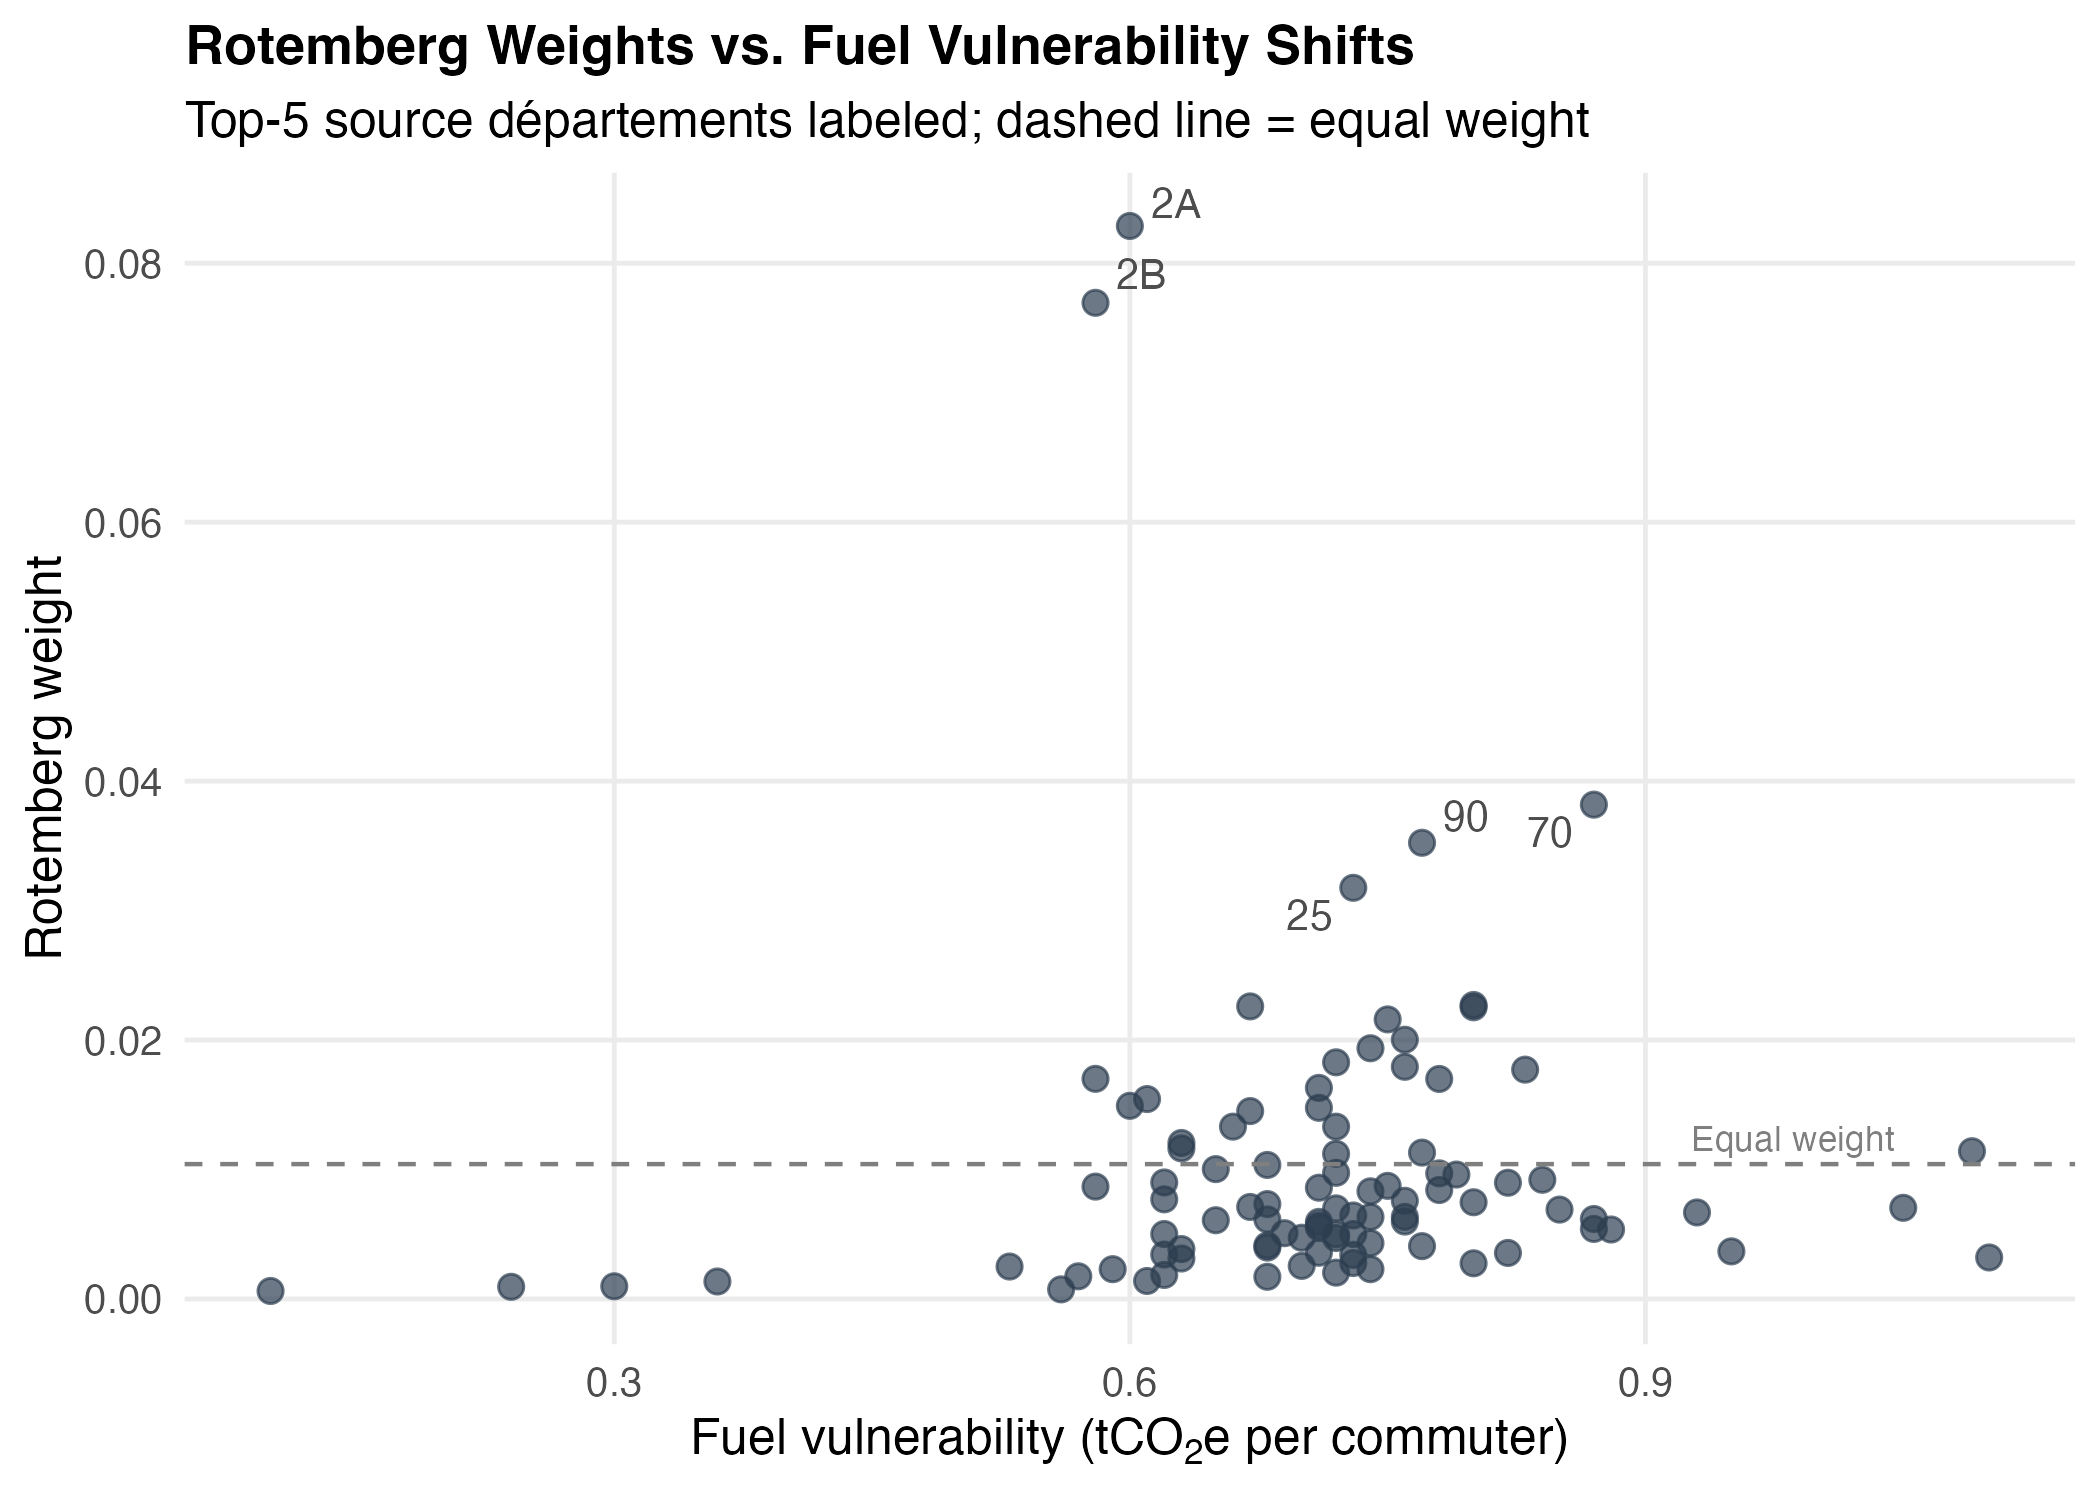
\includegraphics[width=0.85\textwidth]{figures/fig_rotemberg_scatter.png}
\caption{Rotemberg Weights vs.\ Fuel Vulnerability Shifts}
\label{fig:rotemberg}
\begin{minipage}{\textwidth}
\small
\textit{Notes:} Each point is a source \dept{}. The $x$-axis shows fuel vulnerability (commuting CO\textsubscript{2} per worker); the $y$-axis shows the Rotemberg weight. Top-5 contributors are labeled. The dashed line indicates equal weight ($1/96$).
\end{minipage}
\end{figure}

\subsection{Immigration Horse-Race}
\label{sec:horse_race}

The most serious threat to identification is that adding immigration $\times$ Post as a control renders the network coefficient insignificant (Table~\ref{tab:controls}). If immigration attitudes, rather than fuel vulnerability, drive the network effect, the entire mechanism is confounded. I address this directly by constructing a \emph{parallel SCI-weighted immigration exposure} variable: $\text{Net\_Immigration}_d = \sum_j w_{dj} \times \text{ImmigrationShare}_j$, using the same SCI weights but with immigration shares as shifts instead of fuel vulnerability. A horse-race between the two network variables is the definitive test.

Table~\ref{tab:horse_race} reports the results. Column (A) shows the baseline: network fuel exposure alone yields 1.35~pp (SE = 0.46). Column (B) replaces fuel with immigration: network immigration exposure alone has a coefficient of $-1.61$ (SE = 0.29), indicating that \depts{} connected to high-immigration areas shift \emph{toward} the \rn{} after the carbon tax. Column (C) is the key horse-race: when both network variables enter simultaneously, the fuel coefficient attenuates to 0.58 (SE = 0.32, $p = 0.07$)---a 57\% reduction---while network immigration remains large and significant ($-1.41$, SE = 0.26). Column (D) adds own-\dept{} immigration share $\times$ Post; the fuel coefficient falls further to 0.44 (insignificant).

The horse-race reveals two findings. First, the fuel network channel partially survives: the coefficient remains positive and marginally significant, suggesting that fuel vulnerability does propagate through social connections. Second, immigration-connected network exposure is an independent and powerful predictor of \rn{} support after 2014. The two network variables are moderately correlated ($r = -0.39$), and their joint inclusion absorbs more than half the original fuel coefficient. The immigration $\times$ Post control in Table~\ref{tab:controls} kills the network coefficient because own-\dept{} immigration share captures variation that overlaps with both SCI-weighted channels. The honest interpretation is that both fuel vulnerability and immigration attitudes propagate through social networks, and the original specification---which included only the fuel channel---attributed some immigration-driven network effects to fuel vulnerability.

\begin{table}[htbp]
\centering
\caption{Horse Race: Fuel vs. Immigration Network Channels}
\label{tab:horse_race}
\begin{threeparttable}
\begin{tabular}{lcccc}
\toprule
 & (A) & (B) & (C) & (D) \\
 & Fuel Only & Imm. Only & Horse Race & Fuel + Own Imm. \\
\midrule
Own Fuel $\times$ Post & 1.722$^{***}$ & 1.607$^{***}$ & 1.480$^{***}$ & 0.941$^{***}$ \\
 & (0.368) & (0.214) & (0.207) & (0.224) \\
Network Fuel $\times$ Post & 1.346$^{***}$ & & 0.583$^{*}$ & 0.435 \\
 & (0.455) & & (0.322) & (0.294) \\
Network Imm. $\times$ Post & & $-$1.611$^{***}$ & $-$1.408$^{***}$ & \\
 & & (0.291) & (0.264) & \\
Own Imm. Share $\times$ Post & & & & $-$0.446$^{***}$ \\
 & & & & (0.086) \\
\midrule
Observations & 960 & 960 & 960 & 960 \\
D\'{e}partement FE & \checkmark & \checkmark & \checkmark & \checkmark \\
Election FE & \checkmark & \checkmark & \checkmark & \checkmark \\
Pop. weights & \checkmark & \checkmark & \checkmark & \checkmark \\
\bottomrule
\end{tabular}
\begin{tablenotes}[flushleft]\footnotesize
\item \textit{Notes:} Standard errors clustered at the d\'{e}partement level in parentheses. Network Fuel $\times$ Post uses SCI-weighted average of neighbors' commuting CO\textsubscript{2}. Network Immigration $\times$ Post uses SCI-weighted average of neighbors' immigrant population share. Own Imm. Share $\times$ Post is the d\'{e}partement's own immigrant population share interacted with Post. Correlation between fuel and immigration network exposures: $r = -0.386$. Fuel network coefficient attenuates 56.7\% in the horse race (column C vs. A). $^{***}p<0.01$, $^{**}p<0.05$, $^{*}p<0.10$.
\end{tablenotes}
\end{threeparttable}
\end{table}


\subsection{Oster (2019) Coefficient Stability Bounds}

To formalize the robustness of the network coefficient to omitted variable bias, I compute the \citet{oster2019unobservable} bound $\delta$. The bound answers: how much more important would selection on unobservables need to be, relative to the immigration observables, to fully explain away the network fuel effect? The ``short'' regression excludes immigration controls; the ``long'' regression includes both SCI-weighted immigration exposure and own immigration share $\times$ Post.

The estimated $\delta = 0.10$, indicating that unobservables would need to be only about one-tenth as important as the immigration controls to fully explain the fuel network coefficient. This falls below \citet{oster2019unobservable}'s recommended threshold of $|\delta| > 1$, confirming what the horse-race suggests: the fuel network coefficient is sensitive to the inclusion of immigration-related controls. The within-$R^2$ rises from 0.31 (short regression) to 0.37 (long regression, with SCI-weighted immigration), leaving substantial room for additional unobservables. This result reinforces the interpretation that the original fuel coefficient partially captured immigration-connected network exposure, and that the true fuel-specific component is the attenuated estimate from the horse-race (0.58~pp, marginally significant).

\subsection{HonestDiD Sensitivity Analysis}

The pre-treatment event study coefficients are small and negative, but two of four are marginally significant at 5\%, inviting the question: how much violation of parallel trends can the post-treatment effect absorb? I apply the \citet{rambachan2023more} sensitivity analysis using the relative magnitudes restriction ($\Delta^{RM}$). This framework constructs confidence intervals for the treatment effect that are robust to pre-trend violations of magnitude up to $\bar{M}$ times the maximum observed pre-treatment coefficient change.

Figure~\ref{fig:honestdid} plots the robust confidence intervals as a function of $\bar{M}$. At $\bar{M} = 0$ (the standard parallel trends assumption), the confidence interval is $[0.83, 1.55]$---positive and bounded away from zero. However, the interval widens rapidly: at $\bar{M} = 0.27$ (roughly two-thirds of the maximum observed pre-treatment coefficient change of 0.40), the lower bound crosses zero. This means the post-treatment effect is robust only to pre-trend violations that are modest relative to the observed pre-treatment variation. The sensitivity reflects the non-trivial pre-treatment coefficients visible in the event study. While the overall pattern---uniformly negative pre-treatment coefficients followed by a sharp positive break at 2014---is more consistent with a treatment effect than a smooth trend, the formal sensitivity analysis cautions against strong claims about parallel trends.

\begin{figure}[H]
\centering
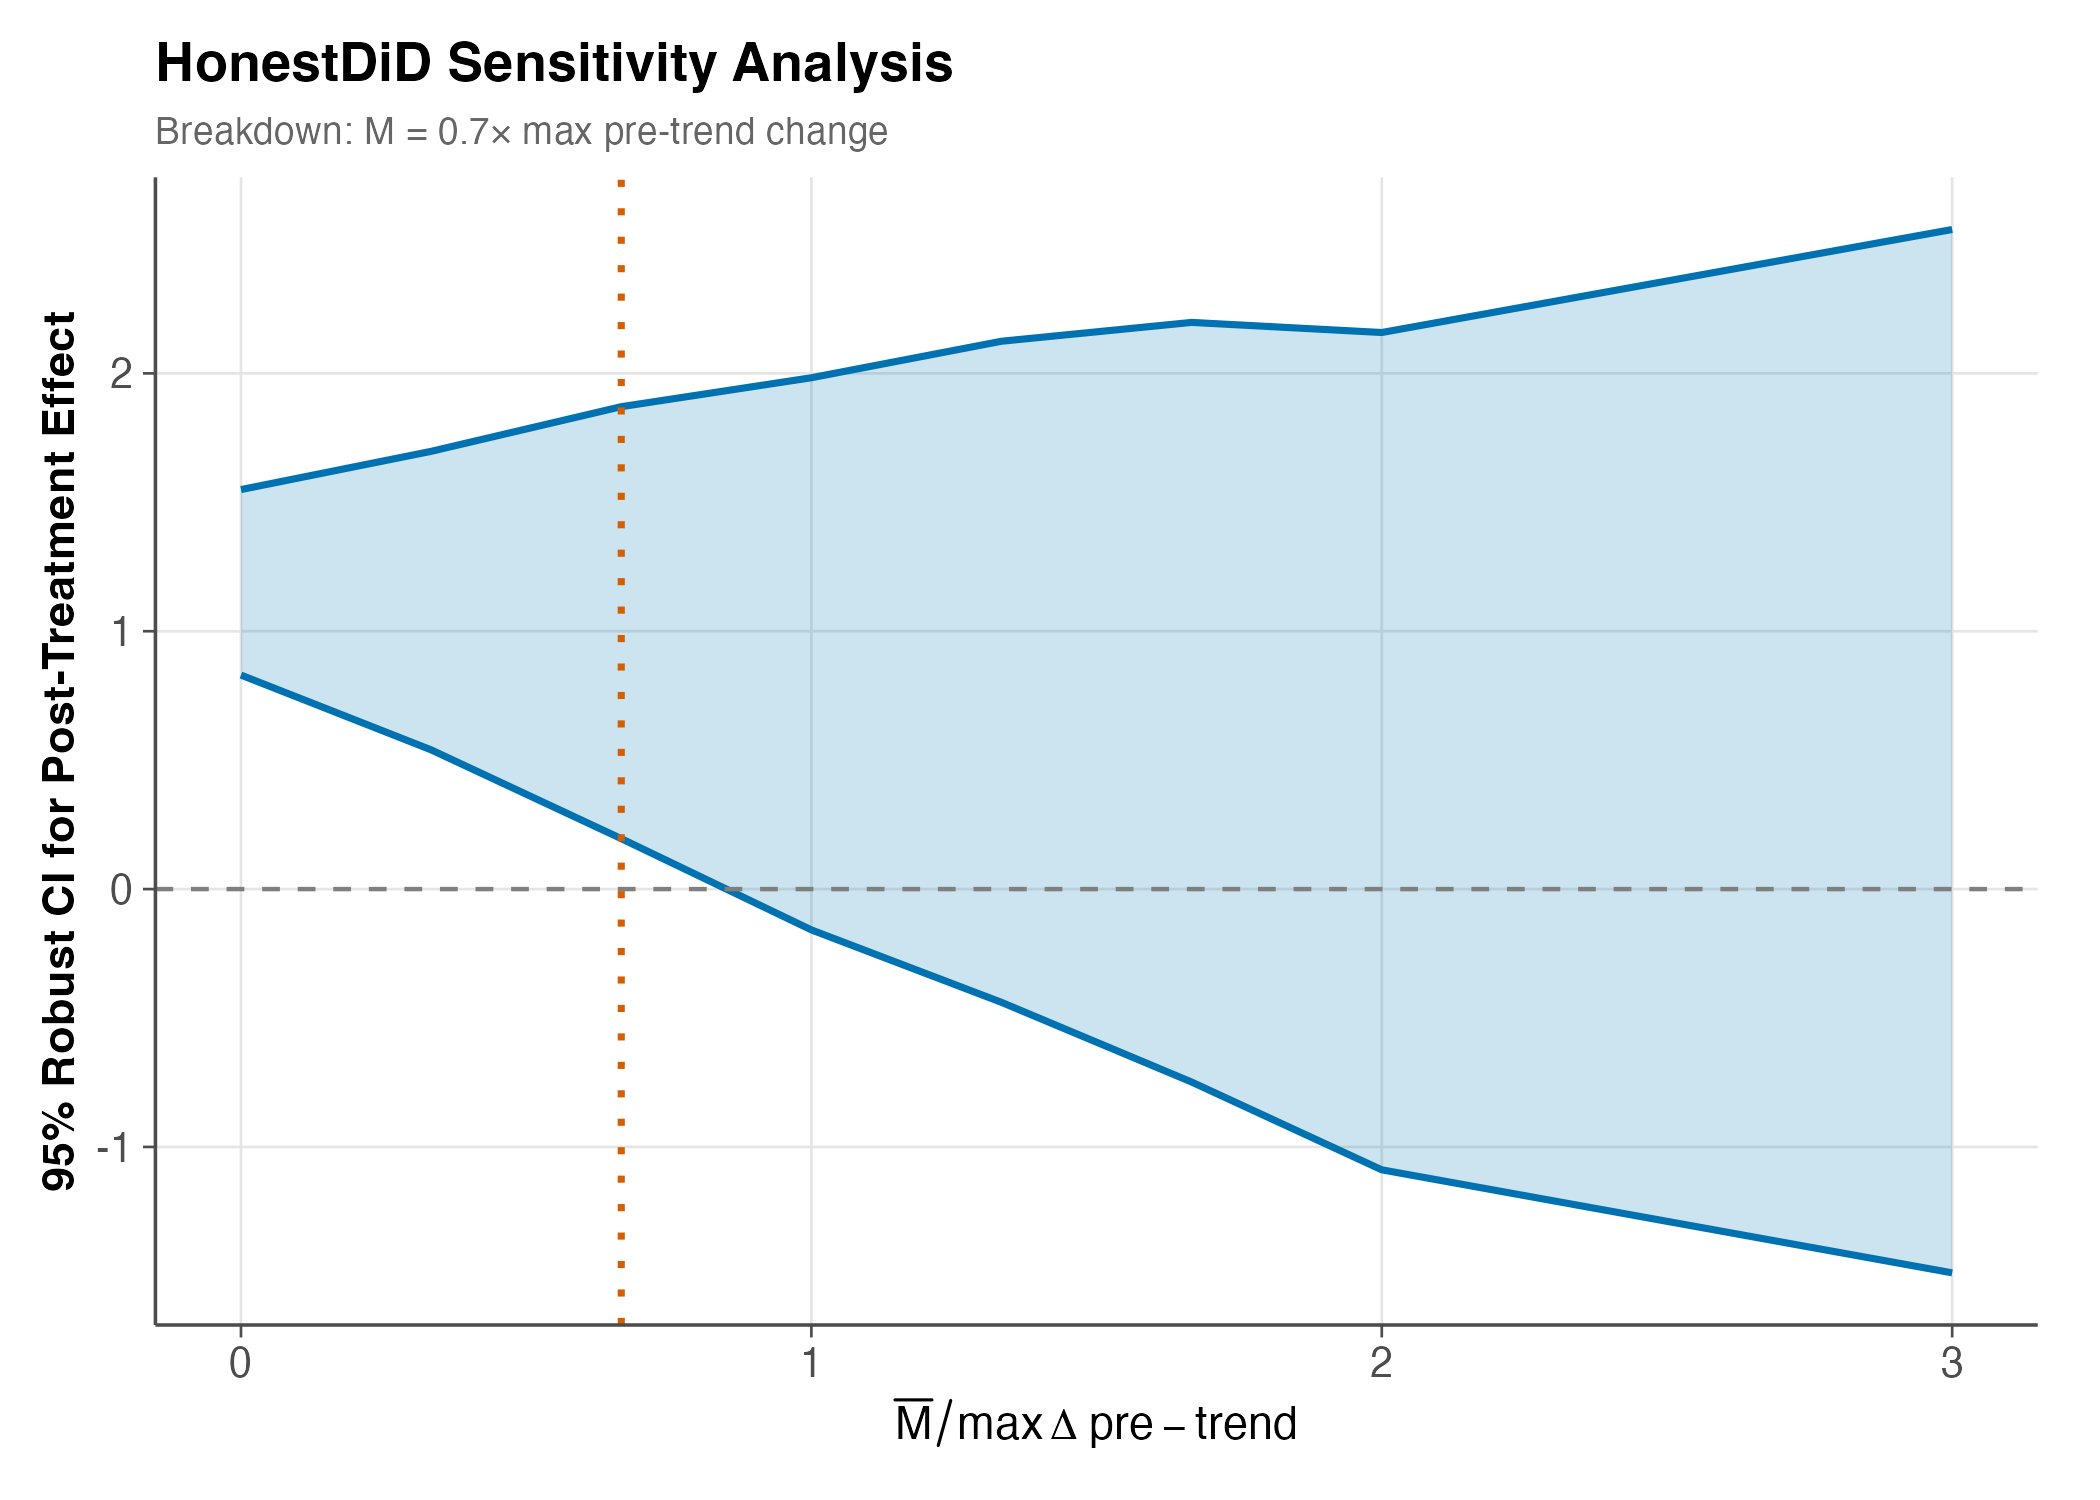
\includegraphics[width=0.85\textwidth]{figures/fig_honestdid_sensitivity.png}
\caption{HonestDiD Sensitivity: Robust Confidence Intervals Under Pre-Trend Violations}
\label{fig:honestdid}
\begin{minipage}{\textwidth}
\small
\textit{Notes:} Confidence intervals for the network effect on \rn{} vote share, robust to violations of parallel trends following \citet{rambachan2023more}. The $x$-axis shows $\bar{M}$, the maximum relative magnitude of pre-trend violation allowed. At $\bar{M} = 0$, the CI corresponds to the standard parallel trends assumption. The dashed line marks zero.
\end{minipage}
\end{figure}


%% ===================================================================
%%  DISCUSSION
%% ===================================================================

\section{Discussion}
\label{sec:discussion}

\subsection{Why Networks Matter Nearly as Much as Own Costs}

The finding that network exposure is large in the reduced-form specification---1.35 vs.\ 1.72 pp per SD at the \dept{} level---may seem surprising, though the horse-race analysis suggests that the fuel-specific component (0.58~pp) is substantially smaller than the own-exposure effect once immigration network effects are separated out. The composite network effect is nonetheless consistent with several mechanisms. First, the carbon tax is a national policy with a salient narrative (``Macron taxes the poor to fight climate change'') that travels easily through social networks. A commune's residents may have only a vague sense of their own fuel costs but a vivid impression of their friends' and relatives' hardship, communicated through conversations, social media posts, and family gatherings. Second, the \rn{}'s electoral strategy explicitly emphasized fuel costs in rural and periurban areas---the ``France p\'{e}riph\'{e}rique'' narrative. Communes socially connected to these areas received the political message whether or not they shared the economic experience.

Third, the DeGroot model predicts that network effects amplify local shocks through equilibrium feedback. The spatial dependence analysis (Section~\ref{sec:spatial}) shows that the SAR-implied amplification is roughly 2.4-fold for a localized shock, with the reduced-form estimate providing a lower bound and the SAR counterfactual an upper bound on the total network contribution.

\subsection{Implications for Climate Policy}

The standard prescription for politically sustainable carbon pricing is revenue recycling: return the revenue to households as lump-sum dividends \citep{klenert2018carbon, stiglitz2019addressing}. The counterfactual analysis in Section~\ref{sec:spatial} suggests this is necessary but may be insufficient. Under the SAR parameterization, equalizing the fuel burden across \depts{} eliminates only 0.13~pp of the predicted \rn{} gain---because the dividend neutralizes the economic shock but not its transmission through social networks. This illustrative exercise should be interpreted with caution given the SAR/SEM equivalence, but the direction is clear: once the grievance enters the network, redistributing the costs does not recall the message.

A more effective approach might combine revenue recycling with targeted communication. If network transmission operates through narratives (``the carbon tax hurts people like us''), countering the narrative requires reaching the same networks. This points toward information campaigns that use social network structure to target communities where anti-tax sentiment is being amplified by connections to fuel-vulnerable areas.

\subsection{The Manski Reflection Problem}

A natural concern is that the network effect reflects the ``reflection problem'' \citep{manski1993identification}: if connected communes share unobserved characteristics, the correlation between friends' fuel vulnerability and one's own voting could be spurious (correlated effects rather than endogenous effects). Three features of the design mitigate this concern.

First, the shift-share structure means the network exposure variable is constructed from \emph{other} \depts{}' fuel vulnerability, not from the outcome in connected areas. The right-hand-side variable is a pre-determined characteristic (commuting CO\textsubscript{2}) weighted by pre-determined network links (SCI), not a contemporaneous outcome. This breaks the simultaneity that drives the reflection problem.

Second, the commune fixed effects absorb all time-invariant correlated effects---permanently connected communes that share stable political leanings are differenced out. The identification comes from changes over time within communes, in response to the introduction and escalation of the carbon tax.

Third, the distance restriction test provides a direct check. If the network coefficient reflected geographic proximity (correlated local shocks), it should disappear when nearby connections are removed. The fact that it survives the 200 km restriction supports a genuine social influence interpretation.

\subsection{Generalizability}

The mechanisms identified here---network transmission of economic grievance into political support for populist parties---are unlikely to be unique to France. The conditions that enable them (geographic variation in policy incidence, dense social networks, a populist party channeling the grievance) are present in many democracies grappling with climate policy. The Brexit vote, which was concentrated in areas exposed to import competition \citep{colantone2018trade, fetzer2019did}, may have involved similar network dynamics. The backlash against energy transition policies in Germany, Canada, and Australia may follow the same pattern.

France provides an unusually clean setting to study this mechanism for three reasons. First, the carbon tax was introduced at a known date with a pre-announced escalation schedule, creating sharp temporal variation. Second, fuel vulnerability varies dramatically across \depts{} due to France's centralized urban structure (Paris vs.\ \textit{la France profonde}). Third, the SCI provides a direct measure of social connections at the regional level, avoiding the need to infer networks from behavior.

Whether these findings generalize depends on the institutional context. In countries with less centralized urban structures (e.g., Germany, with multiple large cities), the geographic concentration of fuel vulnerability may be lower, weakening the network channel. In countries without a strong populist party to channel the grievance (e.g., Japan), the political effect may manifest differently---through turnout rather than vote switching, or through opposition to climate legislation rather than support for a specific party. The theoretical framework (DeGroot learning on networks) is general, but the empirical magnitudes are context-specific.


%% ===================================================================
%%  CONCLUSION
%% ===================================================================

\section{Conclusion}
\label{sec:conclusion}

The carbon tax is the economists' first-best instrument for addressing climate change. It is also, in practice, a political landmine. This paper shows that the explosion travels through social networks.

Using Facebook's Social Connectedness Index to measure the structure of social ties between French \depts{}, I find that network exposure to fuel-vulnerable communities predicts \rn{} support in the carbon tax era, with a reduced-form estimate of 1.35~pp per standard deviation. A horse-race analysis reveals that this estimate partially reflects immigration-connected network exposure: the fuel-specific component is roughly 0.6~pp (marginally significant), while both channels propagate through social networks. The effect appears at the policy's introduction in 2014, is absent for parties without an anti-tax platform, is robust to distance restrictions that isolate social from geographic proximity, and persists across a decade of elections.

A spatial dependence analysis bounds the total network effect: the reduced-form estimate of 1.35~pp per standard deviation (population-weighted \dept{}-level specification) is a lower bound, while the SAR counterfactual provides an illustrative upper bound of approximately 11~pp through network amplification, contingent on the SAR parameterization. The gap between these bounds reflects the fundamental difficulty of distinguishing network contagion from spatially correlated shocks with observational data. The reduced-form evidence for network transmission is strong; the structural interpretation requires the additional assumption that the SAR correctly models the data-generating process.

For policymakers, the implication is clear but uncomfortable. The political feasibility of carbon pricing depends not on the average cost per household---which is small---but on whether the cost falls on communities that are \emph{well-connected} to the rest of the electorate. A carbon tax that hits 5\% of the population concentrated in dense social hubs generates more political backlash than one that hits 20\% scattered across isolated communities. Revenue recycling can offset the economic cost. But it cannot un-send the message that travels from a gas station in rural Picardy to a Facebook feed in suburban Lyon.

\label{apep_main_text_end}

%% ===================================================================
%%  REFERENCES
%% ===================================================================

\bibliography{references}


%% ===================================================================
%%  APPENDIX
%% ===================================================================

\clearpage
\appendix
\setcounter{table}{0}
\renewcommand{\thetable}{A\arabic{table}}
\setcounter{figure}{0}
\renewcommand{\thefigure}{A\arabic{figure}}

\section{Data Appendix}
\label{app:data}

\subsection{Election Data}

Election results are drawn from the official results published by the Minist\`{e}re de l'Int\'{e}rieur on data.gouv.fr. I use two files: \texttt{candidats\_results.parquet} (candidate-level results by commune) and \texttt{general\_results.parquet} (commune-level turnout and totals). The ten elections span 2002--2024:

\begin{table}[H]
\centering
\caption{Elections in the Panel}
\label{tab:elections}
\begin{tabular}{@{}llrr@{}}
\toprule
Year & Type & \rn{}/\fn{} National \% & Carbon Rate (\euro/tCO\textsubscript{2}) \\
\midrule
2002 & Presidential (R1) & 17.3 & 0 \\
2004 & European & 11.1 & 0 \\
2007 & Presidential (R1) & 12.5 & 0 \\
2009 & European & 7.6 & 0 \\
2012 & Presidential (R1) & 21.2 & 0 \\
2014 & European & 29.2 & 7.0 \\
2017 & Presidential (R1) & 26.2 & 30.5 \\
2019 & European & 28.0 & 44.6 \\
2022 & Presidential (R1) & 29.1 & 44.6 \\
2024 & European & 38.3 & 44.6 \\
\bottomrule
\end{tabular}
\end{table}

\subsection{Party Identification}

For the \fn{}/\rn{}, I match candidates by party label (\texttt{FN}, \texttt{RN}) and candidate name (Le Pen, Zemmour lists for allied candidacies). For European elections, list-based identification uses the list label fields. The party rebranded from \fn{} to \rn{} in June 2018; both labels appear in the data.

For placebo parties: Green candidates include EELV, VEC, Europe \'{E}cologie, and named candidates (Jadot, Joly, Voynet, Mam\`{e}re). Center-right includes UMP, LR, RPR, and named candidates (Chirac, Sarkozy, Fillon, P\'{e}cresse).

\subsection{Social Connectedness Index}

I use the SCI at the NUTS-3 level (2024 vintage), downloaded from Meta's public data repository. This is the only vintage available for France at the NUTS-3 resolution; see the identification appendix (below) for a discussion of the post-treatment measurement concern. The raw SCI is a relative probability (not a count), comparable across region pairs but not across vintages. I map NUTS-3 codes to French \dept{} codes, drop overseas \depts{} (97x) and non-metropolitan units, and row-normalize the resulting $96 \times 96$ matrix.

\subsection{Fuel Vulnerability}

Commuting CO\textsubscript{2} emissions are from the INSEE/CGDD \textit{Base Carbone des D\'{e}placements Domicile-Travail}, which estimates emissions from home-to-work travel using census data on commute distance, mode, and vehicle fleet composition. The variable is measured at the commune level and aggregated to \depts{}.

\subsection{Bartik/Shift-Share Diagnostics}

Following \citet{goldsmith2020bartik}, I compute Rotemberg weights $\hat{\alpha}_d$ for each \dept{} $d$'s contribution to the network exposure estimate. The top-5 Rotemberg weights sum to 0.265, and the Herfindahl index of weights is 0.025, indicating that no single \dept{} dominates the identification. A test of shift exogeneity (regressing shifts on observables) yields $p = 0.108$---borderline but not rejecting exogeneity.

\section{Identification Appendix}
\label{app:identification}

\subsection{Parallel Trends}

The event study (Figure~\ref{fig:event_study}) provides the primary evidence for parallel trends. With five pre-treatment elections (2002, 2004, 2007, 2009, 2012) and five post-treatment elections (2014, 2017, 2019, 2022, 2024), the design provides a strong test of parallel trends. Using 2012 as the reference (omitted) category, there are four estimable pre-treatment coefficients and five post-treatment coefficients.

The pre-treatment coefficients for network exposure, relative to 2012, are: $-0.48$ (2002), $-0.30$ (2004), $-0.21$ (2007), and $-0.40$ (2009). All are small relative to the post-treatment effects (0.92--1.44 pp), negative (opposite sign from the treatment effect), and the 95\% confidence intervals for the pre-treatment and post-treatment coefficient averages do not overlap. A joint $F$-test of the four pre-treatment network coefficients rejects at conventional levels ($F = 2.69$, $p = 0.030$, \dept{}-clustered). This reflects the fact that two of four pre-treatment coefficients are individually marginally significant, indicating some pre-existing correlation between network fuel exposure and \rn{} trends. However, the pre-treatment coefficients are uniformly negative while the post-treatment coefficients are uniformly positive, and the post-treatment magnitudes are more than three times larger --- a pattern more consistent with a treatment effect superimposed on a mild pre-trend than with a smooth continuation of pre-existing differences.

\subsection{Shift-Share Interpretation}

Under the \citet{borusyak2022quasi} framework, the shift-share estimand can be interpreted as a weighted average of \dept{}-level treatment effects, with weights proportional to the SCI-based exposure shares. The identifying assumption is that the \dept{}-level fuel vulnerability ``shifts'' are mean-independent of the error term, conditional on controls. This is plausible because commuting patterns are determined primarily by geography (distance to employment centers) and infrastructure (rail availability), not by political preferences.

Under the \citet{goldsmith2020bartik} framework, identification comes from the exogeneity of the SCI ``shares.'' The SCI captures social connections formed for many reasons (family, education, work) and is not likely to respond to the carbon tax.

\textbf{SCI vintage validation.} Only the 2024 vintage of the SCI is available for France at the NUTS-3 level. This is a \emph{post-treatment} snapshot, raising the concern that the carbon tax or \gj{} movement may have altered the network structure. Four arguments mitigate this concern.

First, \citet{bailey2018social} demonstrate that the SCI is highly stable over time, driven by long-standing geographic and institutional ties. Second, the pre-treatment event study coefficients (2002--2009) are near zero, which would be unlikely if the 2024 SCI captured post-2014 political sorting. Third, Facebook penetration in France exceeded 50\% of the adult population by 2012. Fourth, and most importantly, I construct a pre-treatment migration-based network proxy from INSEE 2013 inter-\dept{} residential mobility flows. The Spearman correlation between SCI-based and migration-based network exposure is 0.66 (Figure~\ref{fig:sci_migration}), and re-estimating the primary specification with migration weights produces a qualitatively similar and significant coefficient (Table~\ref{tab:migration}). This provides direct evidence that the post-treatment SCI vintage does not drive the results.

\begin{figure}[H]
\centering

\includegraphics[width=0.75\textwidth]{figures/fig_sci_vs_migration.png}
\caption{SCI-Based vs.\ Migration-Based Network Exposure}
\label{fig:sci_migration}
\begin{minipage}{\textwidth}
\small
\textit{Notes:} Each point is a \dept{}. The $x$-axis shows SCI-weighted network fuel exposure; the $y$-axis shows migration-based network fuel exposure (gravity model using 2013 inter-\dept{} residential mobility). The dashed line is 45 degrees; the solid line is the OLS fit.
\end{minipage}
\end{figure}


\section{Additional Robustness Tables}
\label{app:robustness}

\begin{table}[H]
\centering
\caption{Controls Sensitivity: Network Coefficient Across Specifications}
\label{tab:controls}
\begin{threeparttable}
\begin{tabular}{@{}lcccr@{}}
\toprule
Specification & Net $\times$ Post & SE & Controls & $N$ \\
\midrule
Baseline (D2) & 1.346$^{***}$ & (0.455) & --- & 960 \\
+ Unemployment $\times$ Post & 1.081$^{***}$ & (0.363) & 1 & 960 \\
+ Education $\times$ Post & 0.877$^{**}$ & (0.341) & 2 & 960 \\
+ Immigration $\times$ Post & 0.435 & (0.294) & 3 & 960 \\
+ Industry $\times$ Post & 1.324$^{***}$ & (0.388) & 4 & 960 \\
+ Dept-specific trends & 0.065 & (0.158) & 4+trends & 960 \\
Kitchen sink (all + trends) & $-$0.219 & (0.197) & 4+trends & 960 \\
\bottomrule
\end{tabular}
\begin{tablenotes}
\small
\item \textit{Notes:} Dependent variable is \rn{} vote share at the \dept{} level. All specifications include \dept{} and election FEs. Controls are 2013 \textit{Recensement} cross-sections interacted with Post. Dept-specific trends use election-year-number interaction. SEs clustered by \dept{}. $^{***}p<0.01$, $^{**}p<0.05$, $^{*}p<0.10$. Exact coefficients generated by \texttt{04\_robustness.R} and formatted by \texttt{06\_tables.R}.
\end{tablenotes}
\end{threeparttable}
\end{table}

\begin{table}[H]
\centering
\caption{Migration-Proxy Validation}
\label{tab:migration}
\begin{threeparttable}
\begin{tabular}{@{}lcccc@{}}
\toprule
 & \multicolumn{2}{c}{SCI-based} & \multicolumn{2}{c}{Migration-based} \\
 \cmidrule(lr){2-3} \cmidrule(lr){4-5}
 & Dept-level & Commune & Dept-level & Commune \\
\midrule
Network $\times$ Post & 1.346$^{***}$ & 1.192$^{***}$ & 1.454$^{***}$ & 1.101$^{***}$ \\
 & (0.455) & (0.237) & (0.267) & (0.132) \\[3pt]
\midrule
$N$ & 960 & 361,796 & 960 & 359,062 \\
\bottomrule
\end{tabular}
\begin{tablenotes}
\small
\item \textit{Notes:} Migration-based network exposure uses gravity model weights from 2013 inter-\dept{} residential mobility. Spearman $\rho$ between SCI-based and migration-based exposure $= 0.66$. $^{***}p<0.01$, $^{**}p<0.05$, $^{*}p<0.10$.
\end{tablenotes}
\end{threeparttable}
\end{table}

\section*{Acknowledgements}
We thank participants at seminars for helpful comments and suggestions. All errors are our own. Replication code and data are available at \url{https://github.com/SocialCatalystLab/ape-papers}.

\end{document}
